\chapter{The D-Wave Quantum Computer}


In this second chapter, we aim to understand the D-Wave Quantum systems. In order to achieve that, we start by explaining the basis of quantum annealing that the D-Wave systems used underneath, and how to transform problems into the adequate format for these systems.


\section{Quantum Annealing}


Simulated annealing (SA) is a general optimization technique that was first introduced in 1983 by Kirkpatrick \emph{et al.} \cite{Kirkpatrick1983}. The main idea is to mimic how thermal fluctuations works to let the system escape from local minimums in the cost function. The \emph{temperature} of the system dictates the probability with which the is allowed to jump to worse solutions (higher values of the cost function). The \emph{annealing schedule} is the decrease rate of the temperature, controlled by the programmer. Under the appropriate one, the system would be able to escape from local minimums to reach the global one. If the temperature decreases too quickly, the system converges prematurely to a local minimum. If it decreases too slowly, the technique transforms into a random walker, reaching the global minimum at some point but being worthless time-wise.

Inspiration in thermal fluctuations is used in SA so the system may escape from local minima. Similarly, \emph{quantum tunneling} is used in Quantum Annealing (QA) to escape from local minimums. This new technique was introduced in its present form by two similar proposals \cite{Finnila1994} \cite{Kadowaki1998}.

Quantum tunneling is a quantum mechanical phenomenon where a wavefunction (i.e. a quantum state) may propagate through a potential barrier \cite{Nimtz2008}. The probability of this event occurring depends on the height and width of the barrier (see figure \ref{fig 2.1})

\begin{figure}[h]
	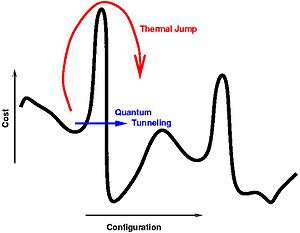
\includegraphics[scale=.8]{QuantumTunneling.jpg}
	\centering
	\caption{Thermal jumps vs quantum tunneling.}
	\label{fig 2.1}
\end{figure}

The main advantage of quantum tunneling compared to classical thermal fluctuations is that the probability of the system shifting depends not only on the height of the potential barrier but also on its width. Thus, the application of QA may potentially outperform SA in problems where the energy (cost) landscape consists of very high and thin barriers surrounding local minimums. 

Particularly, as studied in \cite{Ray1989}, let $\Delta$ be the height of a barrier and $\omega$ its width. The probability of a thermal transition occurring is dictated by $exp\{-\frac{\Delta}{k_B T}\}$ where $T$ and the temperature of the system and $k_B$ is the Boltzmann constant. On the other hand, the probability of a quantum tunneling transition occurring through the same barrier (assuming isolation) is $exp\{-\frac{\sqrt \Delta \omega}{\Gamma}\}$, where $\Gamma$ is an additional constant called the tunneling field \cite{Das2005}. Thus, the probability is much higher for the quantum tunneling effect on high and thin barriers.

We may also observe looking at the previous expressions how the tunneling field and the temperature play similar roles in the different methods. Thus, the annealing schedule of the QA system is controlled using the tunneling field just like the temperature is used in SA.

There are many examples in the literature of QA simulations using classical computers, both theoretical \cite{Morita2008} and numerical -most of them using Quantum Monte Carlo (QMC) methods \cite{Isakov2016} \cite{Farhi2000}-. This evidence suggests the outperformance of SA by simulated QA under certain conditions. It is reasonable to wonder what happens if instead of simulating QA we could somehow encode our problems in a real physical system that tends to its lower energy state (ground state), thus using quantum tunneling naturally. This is precisely what the D-Wave system does.

Let us further deepen into the technicalities of quantum annealing in order to understand how it is implemented in the D-Wave system.


\section{Adiabatic Evolution}
\label{sec:adiabatic-evolution}


The alternative form of the third postulate of quantum mechanics (section \ref{sec:postulate-3}) stated that the evolution of a quantum system is described by the Schrodinger equation:

$$ i \hbar \frac{d|\varphi\ra}{dt} = H|\varphi\ra $$

By better understanding the Hamiltonian $H$ we may control this evolution. Suppose that the evolution of a given quantum system is described by a Hamiltonian $\hat H(t)$. Suppose that at some initial time $t_0$ our quantum system is in an eigenstate $|\varphi(t_0)\ra$ of $\hat H(t_0)$. Since the evolution is continuous, at some other time $t_1 > t_0$ we could expect our system to be in the corresponding eigenstate $|\varphi(t_1)\ra$ of $\hat H(t_1)$. This fact critically depends on the time $\tau = t_1 - t_0$ during which the modification takes place, as stated by the adiabatic theorem, first proposed by Max Born and Vladimir Fock (1928) \cite{Born1928}.

\begin{theorem}[Adiabatic Theorem]
	\label{th:adiabatic-theorem}
	A physical system remains in its instantaneous eigenstate if a given perturbation is acting on it slowly enough and if there is a gap between the eigenvalue and the rest of the Hamiltonian's spectrum.
\end{theorem}

Thus, we may define diabatic and adiabatic processes depending on how they adapt to the system changes \cite{Kato1950}.

\begin{definition}
	A \emph{diabatic process} is a process where rapidly changing conditions prevent the system from adapting its configuration during the process. Typically there is no eigenstate of the final Hamiltonian with the same functional form as the initial state. The system ends in a linear combination of the states.
\end{definition}

\begin{definition}
	An \emph{adiabatic process} is a process where gradually changing conditions allow the system to adapt its configuration. If the system starts in an eigenstate of the initial Hamiltonian, it will end in the corresponding eigenstate of the final Hamiltonian.
\end{definition}

The 'gap condition' that appears in theorem \ref{th:adiabatic-theorem} refers to an additional requirement: the spectrum of $\hat H(t)$ is \emph{nondegenerate}, meaning there are no two equal eigenvalues at fixed time $t$. This condition is also called the \emph{no-crossing} condition and allows us to sort the eigenstates using the eigenvalues without any ambiguity.

As a classical analogy for adiabatic evolution, consider a simple pendulum. If the pendulum's support point is moved, the oscillation of the pendulum may change. In fact, violent changes on the support point will dramatically affect the pendulum's movement, changing it completely. However, if the support point is moved slowly enough, the pendulum will remain unchanged. These are examples of diabatic and adiabatic processes respectively.


\subsection{Avoided crossing}


Let us consider an important physical example known as the \emph{avoided crossing} \cite{Cohen-Tannoudji2006}. Consider a two-state quantum system, i.e. a qubit. Suppose its Hamiltonian to be:

$$
	H = 
	\begin{pmatrix}
		E_1 & 0 \\
		0 & E_2 
	\end{pmatrix}
$$

Whose eigenvalues are $E_1$ and $E_2$, and eigenvectors,

$$
	|0\ra = 
	\begin{pmatrix}
	1 \\
	0 
	\end{pmatrix}, \quad
	|1\ra = 
	\begin{pmatrix}
	0 \\
	1 
	\end{pmatrix}
$$

which will be used as our base. Thus, a state vector describing the system may be written as a superposition of both states:

$$ |\varphi\ra = \alpha|0\ra + \beta|1\ra $$

Supposing adiabatic evolution, if the system is prepared in either one of the eigenstates it will remain as such as long as the gap condition is sufficed: $E_1 \neq E_2$. However, if $E_1 = E_2$, any superposition of states will be an eigenstate, thus remaining unchanged. Hence, independently of $E_1$ and $E_2$, any system prepared in an eigenstate will remain as such, supposed adiabatic evolution.

Let us consider a perturbation $P$ into our original system. For simplicity, we only consider perturbations with degenerated diagonal. Our new Hamiltonian will be the following:

$$
	H' = H + P =
	\begin{pmatrix}
	E_1 & 0 \\
	0 & E_2 
	\end{pmatrix} +
	\begin{pmatrix}
	0 & \omega \\
	\overline \omega & 0 
	\end{pmatrix} = 
	\begin{pmatrix}
	E_1 & \omega \\
	\overline \omega & E_2 
	\end{pmatrix}
$$

where $\omega \in \C$. Note that by setting $\omega$, the other value in the antidiagonal is fixed since $H'$ must be Hermitian. By using the characteristic equation we may compute the eigenvalues of $H'$:

$$ E_+ = \frac{1}{2}(E_1 + E_2) + \frac{1}{2}\sqrt{(E_1 - E_2)^2 + 4|\omega|^2} $$
$$ E_- = \frac{1}{2}(E_1 + E_2) - \frac{1}{2}\sqrt{(E_1 - E_2)^2 + 4|\omega|^2} $$

We may plot $E_+$ and $E_-$ along the vertical axis while varying $(E_1 - E_2)$ in the horizontal axis, and find two branches of a hyperbola. The curves asymptotically approach the original unperturbed states $E_1$ and $E_2$. Analyzing the curves and the previous equations it becoms evident that the new energy staes are no longer equal, even if the original states were degenerate ($E_1 = E_2$). However, if the pertubation is removed, $\omega = 0$, if may find that where the states are degenerate and $(E_1 - E_2) = 0$, the new eigen become equal, $E_+ = E_-$ and the levels cross. Thus, by adding a perturbation efffect, these level crossing are completely avoided.

In the table of figures \ref{fig:avoided-crossing}, we find a series of plots describing this behavior for different values of $\omega$. The eigenvalues have been set to $E_1 = -E_2$ (thus $E_1 + E_2 = 0$) for simplicity. We can see how as the perturbation $\omega$ becomes smaller, the hyperbola branches adjust better to the original states and the gap becomes thinner and thinner. Finally, when the perturbation is removed, the levels cross. The reader may find an interactive representation using GeoGebra in \cite{GeoGebra-AvoidedCrossing}.

\begin{table}[H]
	\centering
	\makebox[\textwidth][c]{
		\begin{tabular}{cc}		
			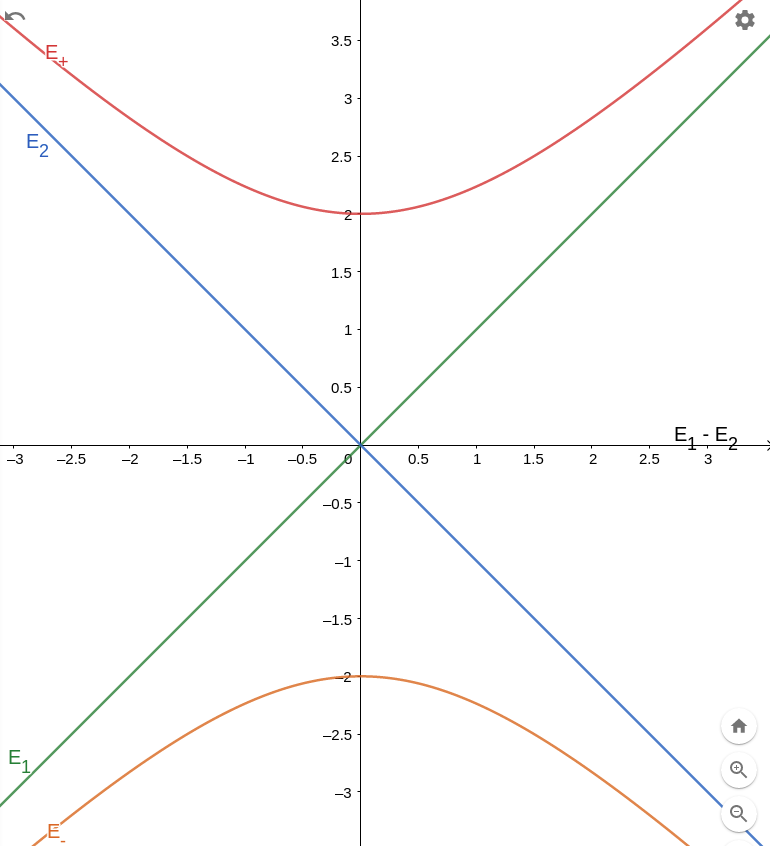
\includegraphics[scale=0.2]{geogebra1.png} &
			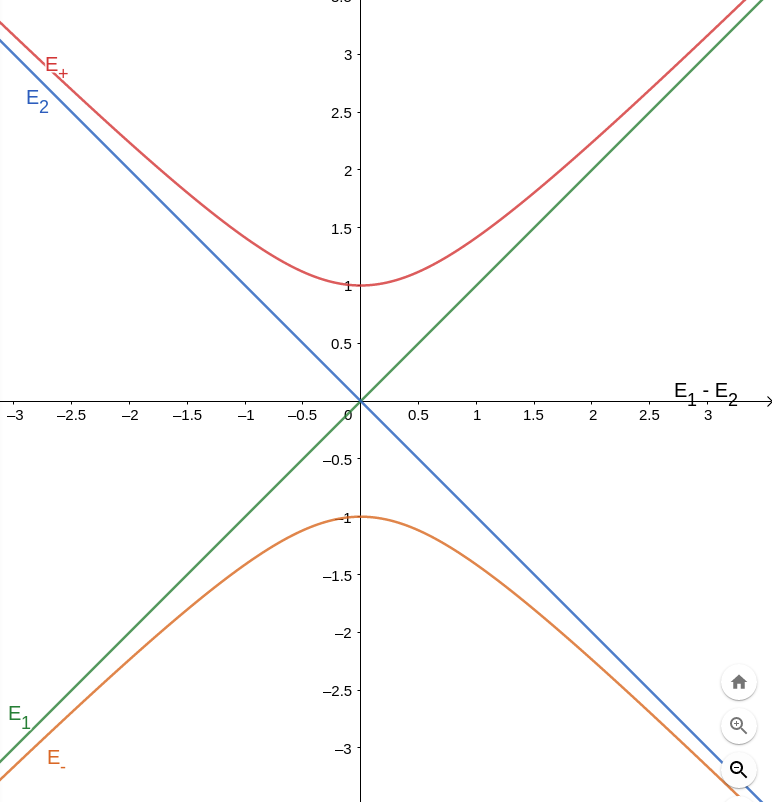
\includegraphics[scale=0.2]{geogebra2.png} \\
			
			$\omega = 1$ & $\omega = 0.5$ \\
			
			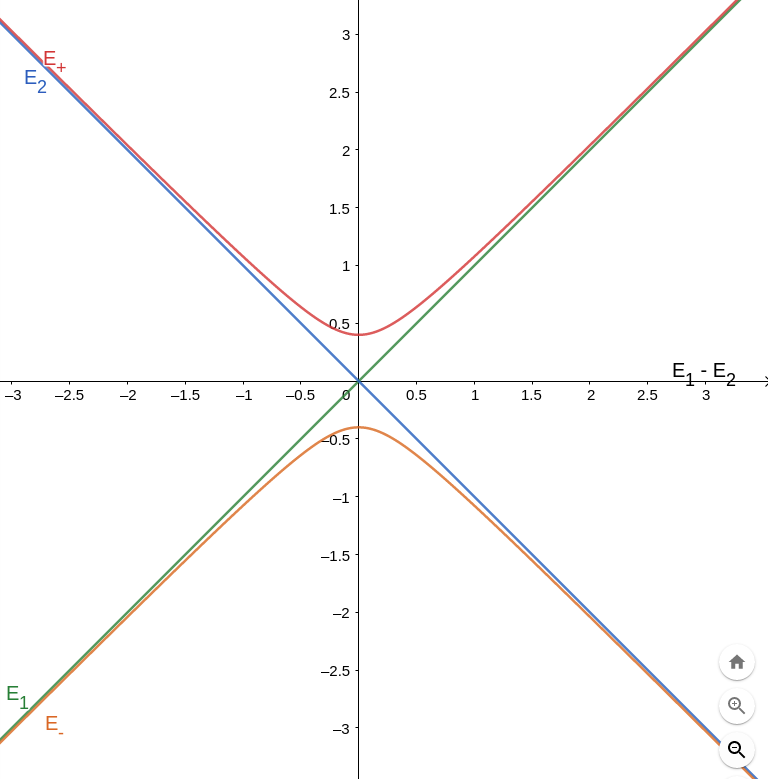
\includegraphics[scale=0.2]{geogebra3.png} &
			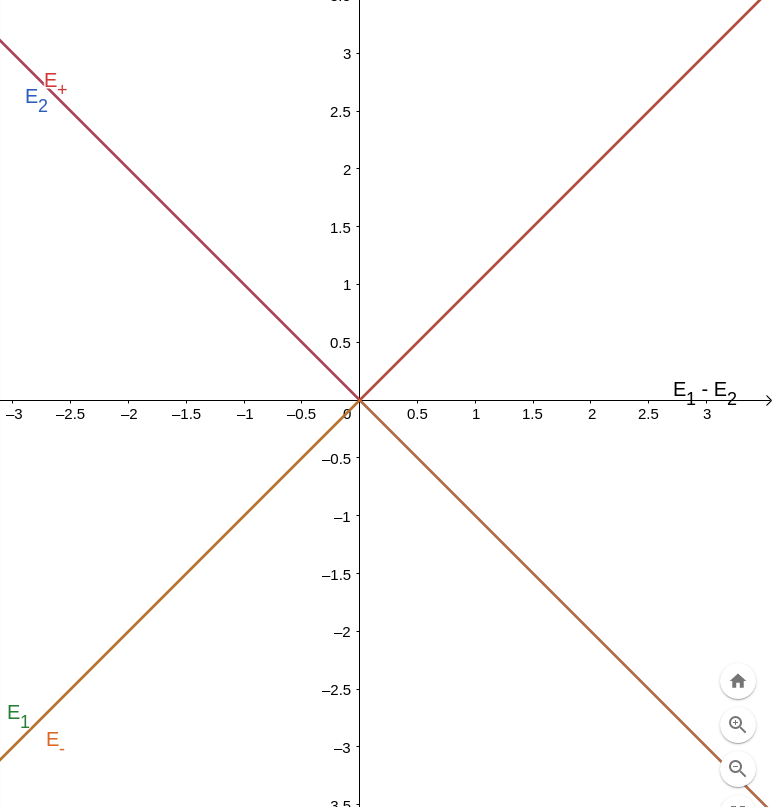
\includegraphics[scale=0.2]{geogebra4.png}  \\
			
			$\omega = 0.2$ & $\omega = 0$ \\
		\end{tabular}
	}
	\caption{Avoided crossing in two-state system \cite{GeoGebra-AvoidedCrossing}. By increasing the perturbation $\omega$, the energy level crossing is avoided. }
	\label{fig:avoided-crossing}
\end{table}

In the case of a single qubit, the two original states $|0\la$ and $|1\ra$ are never degenerate by our definition, so the crossing does not occur with or without a perturbation.

The implications of energy level crossing in quantum annealing will be better explained in section \ref{sec:quantum-annealing-dwave}. For now, it suffices to now that avoided crossing in energy levels is a strongly desired hypothesis that in practice is difficult to fulfill. It will be partially responsible for suboptimality in the use of quantum annealing.


\subsection{Solving problems using adiabatic evolution}


In order to use adiabatic evolution to solve optimization problems we will configure our own Hamiltonian for the system. In particular, the Hamiltonian will be a time-dependent linear combination of two constant Hamiltonians:

$$ H(t) = f(t) \cdot H_{initial} + g(t) \cdot H_{final} \quad \forall t \in [t_{initial}, t_{final}] $$

where $f,g: [t_{initial}, t_{final}] \longrightarrow \R^+_0$. The initial Hamiltonian, $H_{initial}$, will be an easy configuration so we may prepare our system to start in the ground state of $H_{initial}$. The final Hamiltonian, $H_{final}$, will encapsulate the cost function of our problem such that the minimum value is reached in the ground state. 

Functions $f$ and $g$ fulfill that $g(t_{initial}) = f(t_{final}) = 0$. When times elapses and supposing adiabatic evolution, the system will stay on the ground state of $H$ and by $t = t_{final}$, the system will be in the $H_{final}$'s ground state, codifying the minimum of our cost function.

However, we cannot always grant the necessary conditions for perfect adiabatic evolution. In some cases, the gap condition does not suffice as the system will jump with a certain probability to other eigenstates, providing suboptimal solutions which are still useful. This depends on the eigenvalues of the final Hamiltonian, which at the same time entirely depends on the problem being studied.

The only question remaining is how to encode our cost function in a Hamiltonian.


\section{QUBO and Ising models}


The QUBO and Ising models can be easily represented with a Hamiltonian. In practice, non-optimization problems are transformed into optimization problems and then codified as either QUBO or Ising to be solved using quantum annealing. Let us explore these types of problems and some examples of these transformations.

Let $B = \{0,1\}$ and $f_Q: \B^n \longrightarrow \R $ be a quadratic polynomial over binary variables:

$$ f_Q(x) = \sum_{i=1}^n \sum_{j=1}^i q_{ij} x_i x_j $$

where $x_i \in \B$ for $i \in \{1, \cdots, n\}$ and the coefficients $q_{ij} \in \R$ for $1 \leq j \leq i \leq n$. A \textbf{quadratic unconstrained binary optimization (QUBO) problem} consists of finding a binary vector $x'$ such that $x'$ is a minimum of $f_Q$:

$$ x' = \underset {x \in \B^n }{\arg \min} ~ f_Q(x) $$

QUBO problems can be formulated in a more compact matrix form:

$$ f_Q(x) = x^T Q x $$

where $Q$ is a $n \times n$ symmetric matrix containing $q_{ii}$ and its diagonal and $q_{ij} / 2$ in position $(i,j)$ where $i \neq j$. Let us explore some simple properties of QUBO problems:

\begin{itemize}
	\item Multiplying the coefficients $q_{ij}$ by a constant $a \in \R^+$ scales the output by exactly $a$. Thus, $x'$ remains the minimum:
	
		$$ f_{aQ}(x) = \sum_{i<j} (a q_{ij}) x_i x_j  = a \sum_{i<j} q_{ij} x_i x_j = a f_Q(x) $$
		
	\item Flipping the sign of the coefficients flips the sign of $f_Q(x)$. Thus, $x'$ is the maximum of $f_{-Q}(x)$
	
		$$ f_{-Q}(x) = \sum_{i<j} (-q_{ij}) x_i x_j  = - \sum_{i<j} q_{ij} x_i x_j = -f_Q(x) $$
		
	\item If all coefficients are positive the minimum is $x = (0, \ldots, 0)$. Analogously, if all coefficients are negative, the minimum is $x = (1, \ldots, 1)$. 
\end{itemize}

When the dependendy on $Q$ is obvious, it may be left implicit by writting our cost function simply as $f$.

The \textbf{Ising models}, on the other hand, find their inspiration in physics. They are named after the physicist Ernst Ising who solved the one-dimensional model in his 1924 thesis \cite{Ising1924}. They are stated using a Hamiltonian function $H: \{-1, 1\}^n \longrightarrow \R$:

$$ H(\upsigma) = - \sum_{\la i ~ j \ra} J_{ij} \upsigma_i \upsigma_j - \mu \sum_j h_j \upsigma_j $$

with parameters $h_j, J_{ij}, \mu \in \R$. The \emph{spin variables} $\upsigma_i$ are in $\{-1, 1\}$ instead of $\B$. Moreover, the spin variables are arranged in a graph, typically a \emph{lattice}, where a local structure repeats periodically. The only pair of variables $\la i ~ j \ra$ which are neighbor nodes in the graph may have non-zero coefficients $J_{ij}$. Let us see the connection between the QUBO and Ising models by using the identity $\upsigma \mapsto 2x -1$:

\begin{equation*}
	\begin{split}
		f(x)	& = \sum_{\la i ~ j \ra} - J_{ij} (2x_i - 1) (2x_j - 1) - \sum_j \mu h_j (2x_j - 1) \\
				& = \sum_{\la i ~ j \ra} - 4J_{ij} x_i x_j + 2J_{ij} x_i + 2J_{ij} x_j - J_{ij} + \sum_j 2 \mu h_j x_j - \mu h_j \qquad \text{using }  x_j = x_jx_j \\
				& = \sum_{i=1}^n \sum_{j=1}^i q_{ij} x_i x_j + C
	\end{split}
\end{equation*}

where 

\begin{equation*}
	q_{ij} = 
		\begin{dcases}
			-4 J_{ij} 																	& \text{if } i \neq j \\
			\sum_{\la k ~ i \ra} 2 J_{ki} + \sum_{\la i ~ l \ra} 2 J_{il} + 2 \mu h_i	& \text{if } i = j
		\end{dcases}
\end{equation*}

$$ C = - \sum_{\la i ~ j \ra} J_{ij} - \mu \sum h_j $$

Since adding a constant does not change the minimum $x'$, it can be omitted during optimization and only be used for transforming one type of problem into another.

In practice, a given problem would be translated into either QUBO or Ising. It is useful to learn both types of problems since they both are popular in the literature. Let us deepen in the translation of different NP problems. The resolution of QUBO and Ising models will not be studied, but only the translations into these models. In particular, these examples of QUBO transformations are from \cite{Glover2019} and \cite{Lucas2014} unless stated otherwise. For an extensive literature review on QUBO and Ising translations of NP problems, refer to \cite{Kochenberger2014}.


\subsection{The Max Cut problem}


One of the first famous problems that was encoded as a QUBO was the max-cut problem due to its natural translation. It reads as follows: Given an undirected graph $G(V, E)$ with vertex set $V$ and edge set $E$, seek a partition of $V$ such that the number of edges between both sets is as large as possible.

The max-cut problem can be modeled by setting variable $x_j = 1$ if vertex $j$ is in one set and $x_j = 0$ if it is in the other one, for every vertex $j$ in $V$. The quantity $(x_i + x_j - 2 x_i x_j)$ marks whether the edge $(i,j)$ is in the cut. That is, $(x_i + x_j - 2 x_i x_j) = 1$ if the vertices $x_i$ and $x_j$ are in different sets, and $0$ otherwise.

Thus, maximazing the number of edges in the cut is encoded as a QUBO as:

$$ \text{Maximize } f(x) = \sum_{(i,j) \in E} \big( x_i + x_j - 2 x_i x_j \big) $$


\newparagraph{Numerical example}


Consider the following graph:

\begin{figure}[H]
	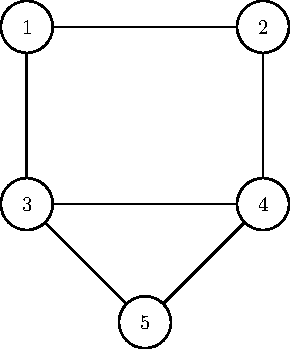
\includegraphics[scale=1]{graphs/max-cut-example.pdf}
	\centering
\end{figure}

We would have five variables: $x_1, \cdots, x_5$. The cost associated to edge $(1,2)$ is $x_1 + x_2 - 2 x_1 x_2$. By repeating this process for every edge in the graph we obtain the cost function:

$$ \text{Maximize  } f(x) = (x_1 + x_2 - 2 x_1 x_2) + (x_1 + x_3 - 2 x_1 x_3) + (x_2 + x_4 - 2 x_2 x_4) $$
$$ +(x_3 + x_4 - 2 x_3 x_4) + (x_3 + x_5 - 2 x_3 x_5) + (x_4 + x_5 - 2 x_4 x_5) $$

or equivalently:

$$ \text{Maximize  } f(x) = 2x_1 + 2x_2 + 3x_3 + 3x_4 + 2x_5$$ 
$$ - 2x_1x_2 - 2x_1x_3 - 2x_2x_4 - 2x_3x_4 - 2x_3x_5 - 2x_4x_5 $$

We can transform the problem using the following symmetric matrix:

$$
	Q = 
	\begin{pmatrix}
	2 & -1 & -1 & 0 & 0 \\
	-1 & 2 & 0 & -1 & 0 \\
	-1 & 0 & 3 & -1 & -1 \\
	0 & -1 & -1 & 3 & -1 \\
	0 & 0 & -1 & -1 & 2
	\end{pmatrix}
$$

Yielding the following compact form:

\begin{equation}
\ref{eqn:max-cut-function}
	\text{Maximize  } f_Q(x) = x^T Q x
\end{equation}

Keep in mind that quadratic elements in the cost function are divided by two when added to the $Q$ matrix, since after multiplying and adding in equation \ref{eqn:max-cut-function} they appear twice.

By solving this model using quantum annealing we obtait the minimum value of $f_Q(x)$: $x = (0, 1, 1, 0, 0)$. Thus, vertices $2$ and $3$ are in one set and vertices $1$, $4$ and $5$ are in the other one.


\subsection{General translation method}

The previous problem was naturally transformed into QUBO due to its particular constraints. However, can any quadratic optimization problem be encoded as a QUBO?

The answer to this question is positive. Furthermore, any quadratic optimization problem with linear constraints may be transformed into a QUBO. Let us first study a simple case. Consider the following problem:

\begin{gather*}
	\text{Minimize } f(x_1, x_2) \\
	\text{subject to the constraint} \\
	x_1 + x_2 \leq 1
\end{gather*}

where $x_1, x_2 \in \B$. We may transform our linear constraint into a penalty $P(x_1x_2)$ for some positive scalar $P$. This term equals $0$ if and only if our constraint is satisfied by the variables. Thus, by adding the penalty to our cost function, for $P$ large enough, the problem

\begin{gather*}
	\text{Minimize } f(x_1, x_2) + Px_1x_2
\end{gather*}

will minimize $f(x_1, x_2)$ and, at the same time, satisfy the constraint. Namely, the constraint translates into adding a non-negative value to the cost function. Some other useful translations can be found in table \ref{tab:penalties-table}. In general, if the cost function is being minimized we may substitute constraints by non-negative terms that only equal zero if they are satisfied, multiplied by a large enough positive value $P$. Thus, we may remove the associated constraints by simply adding these terms to the cost function.

\begin{table}[h]
	\centering
	\begin{tabular}{cc}
		Classical Constraint 		& Equivalent Penalty   			\\ \hline
		$x + y \leq 1$       		& $P(xy)$              			\\
		$x + y \geq 1$       		& $P(1 - x - y + xy)$  			\\
		$x + y = 1$          		& $P(1 - x - y + 2xy)$ 			\\
		$x \leq y$       			& $P(x - xy)$      
		
		   			\\
		$x_1 + x_2 + x_3 \leq 1$	& $P(x_1x_2 + x_1x_3 + x_2x_3)$	\\
		$x = y$              		& $P(x + y - 2xy)$    
	\end{tabular}
	\caption{Constraints and penalties relations}
	\label{tab:penalties-table}
\end{table}

Specifically, let us study the more general case:

$$ \text{Minimize } f(x) = x^T C x $$
$$ \text{subject to the constraints} $$
$$ Ax = b $$

where $x \in \B^n$, $k$ is the number of constraints, $b \in \R^k$, $C$ is a $n \times n$ real matrix and $A$ is a $k \times n$ real matrix. This accomodates to both linear and quadratic cost function since elements in the diagonal are $c_{ii} x_i^2 = c_{ii} x_i$. For a positive scalar $P$, the quadratic penalty $P (Ax - b)^T (Ax - b)$ is added to the cost function to obtain:

\begin{equation*}
	\begin{split}
		f'(x)	& = x^T C x + P (Ax - b)^T (Ax - b) \\
		& = x^T C x + P (x^TA^TAx - \cancelto{}{x^TA^Tb} - \cancelto{}{b^TAx} + b^Tb) \\
		& = x^T C x + x^T D x + c \\
		& = x^T Q x + c 
	\end{split}
\end{equation*}

where $D = P(A^TA)$, $c = P(b^Tb)$ and $Q = C + D$. Since the constant $c$ does not affect where the minimum is reached, $f$ and $f'$ share this minimum. Therefore, we may simply solve:

$$ \text{Minimize } f(x) = x^T Q x $$

which is a QUBO problem.

In this development, we only considered equality constraints. There is also a general method to transform inequality constraints into equality ones by introducing \emph{slack variables} \cite{Hull2003}. In practice, the general case will not be necessary since the constraints are usually quite simple.

Finally, we may also consider satisfiability problems. That is, given a set of constraints for the variables, find a configuration of them such that all the constraints are satisfied. If the constraints are linear, these problems may be transformed into QUBO by setting the cost function as constant and following the same method. Suppose the constraints over $x$ can be written as $Ax = b$. The equivalent optimization problem is written as:

$$ \text{Minimize } f(x) = 0 $$
$$ \text{subject to the constraints} $$
$$ Ax = b $$

Any solution satisfying the constraint will yield $0$ on the penalties, thus minimizing the transformed cost function $f'(x) = x^T Q x$. 

Let us explore some more complicated examples to expand on these ideas.


\subsection{Satisfiability problems: Max 2-SAT}


This example is based on \cite{Glover2019} and \cite{Farhi2000}.

In the previous section, we mentioned satisfiability problems, also known simply as SAT. In this section, we study these problems from its traditional logic perspective.

A \emph{clause} is statement depending on a finite set of binary variables , $C = C(x_1, \ldots, x_k)$, that be either True or False. A \emph{literal} is a variable or its negation: $x$ and $\neg x$ are literals. Let $C_1, \ldots, C_n$ be a set of \emph{Clauses} depending on variables $x_1, \ldots, x_m$. The satisbiality problem associated to this problem is to find a configuration for the variables $x_1, \ldots, x_m$ such that every clause is true:

$$ C_1 \wedge \cdots \wedge C_n $$

SAT was the first problem proven to be NP-complete. This result is known as the Cook-Levin theorem, named after Stephen Cook and Leonid Levin \cite{Book1980}. Its relevance in computer science is astronomical. There have been many variations of SAT problems, let us explore one of them, the Max 2-SAT variation, and transform it into a QUBO model.

Max 2-SAT problem is an optimization problem. Its main restriction is that each clause may depend on at most two literals and it is true if and only if at least one literal is true. The problem consists of finding a configuration of variables such that the number of true clauses is maximized. Each clause $C(x_C, y_C)$ is associated with an energy function depending on the variables $(x_C, y_C)$:

\begin{equation*}
E_C(x_C, y_C) = 
\begin{dcases}
0,	& \text{if } (x_C, y_C) \text{ satisfies clause } C \\
1,	& \text{if } (x_C, y_C) \text{ violates clause } C \\
\end{dcases}
\end{equation*}

The energy of the whole system, which will work as our cost function, is defined as the sum of all the energies:

$$E = \sum_C E_C$$

Clearly $E \geq 0$ and $E = 0$ if and only if every clause is true. Furthermore, the minimum energy of the system $E_0$ will be reached where the maximum number of clauses are satisfied: exactly every clause but $E_0$ will be true. Note that this perspective does not depend on the Max 2-SAT problem. In fact, the same process is used to transform other satisfiability problems.

The remaining question is how to transform our clauses into energy functions. For the Max 2-SAT problem this is quite straightforward. Each clause may depend on at most two literals. Thus, there are either zero, one, or two negations in each clause. We may study this cases separately, as seen in table \ref{tab:penalties-max-2-sat-table}.

\begin{table}[h]
	\centering
	\begin{tabular}{ccc}
		Clause 					& Traditional constraing	& Energy function		\\ \hline
		$x \vee y$       		& $x + y \geq 1$    		& $(1 - x - y + xy)$	\\
		$\neg x \vee y$      	& $\neg x + y \geq 1$ 		& $(x - xy) $  			\\		
		$\neg x \vee \neg y$    & $\neg x + \neg y \geq 1$ 	& $(xy)$ 
	\end{tabular}
	\caption{Clause and energy functions relations}
	\label{tab:penalties-max-2-sat-table}
\end{table}

Since every energy function is quadratic, the total energy will also be quadratic. This is the cost function used in our QUBO model:

$$ \text{Minimize } E(x) = \sum_C E_C$$

Note that, interestingly enough, our QUBO model does not depend on the number of clauses but only on the number of variables. This means that a problem with $30.000$ clauses and $200$ variables will only use $200$ variables in the associated QUBO model.


\newparagraph{Numerical Example}


Given the following set of clauses found in table \ref{tab:penalties-max-2-sat-example}, find a solution to the Max 2-SAT problem associated with them.

\begin{table}[h]
	\centering
	\begin{tabular}{ccc}
		Clause $\#$	& Clause						& Energy function				\\  		\hline
		1       	& $x_1 \vee x_2$    			& $(1 - x_1 - x_2 + x_1x_2)$	\\
		2       	& $x_1 \vee \neg x_2$    		& $(x_2 - x_1x_2)$				\\
		3       	& $\neg x_1 \vee x_2$    		& $(x_1 - x_1x_2)$				\\
		4       	& $\neg x_1 \vee \neg x_2$    	& $(x_1x_2)$					\\
		5       	& $\neg x_1 \vee x_3$    		& $(x_1 - x_1x_3)$				\\
		6		  	& $\neg x_1 \vee \neg x_3$    	& $(x_1x_3)$					\\
		7       	& $x_2 \vee \neg x_3$    		& $(x_3 - x_2x_3)$				\\
		8       	& $\neg x_2 \vee x_3$    		& $(x_2 - x_2x_3)$				\\
		9       	& $\neg x_2 \vee \neg x_3$    	& $(x_2x_3)$					\\
		10       	& $x_2 \vee x_4$    			& $(1 - x_2 - x_4 + x_2x_4)$	\\
		11       	& $x_3 \vee x_4$    			& $(1 - x_3 - x_4 + x_3x_4)$	\\
		12       	& $\neg x_3 \vee \neg x_4$    	& $(x_3x_4)$					
	\end{tabular}
	\caption{Clause and energy functions relations}
	\label{tab:penalties-max-2-sat-example}
\end{table}

A quick look at the first four clauses tells us that we cannot possibly find a configuration of variables that satisfy every clause. In fact, at most three of those four will be true. Adding the energies associated with every clause gives us the energy of the system, and therefore our QUBO model:

$$ \text{Minimize } E(x) = 3 + x_1 - 2 x_4 - x_2x_3 + x_2x_4 + 2 x_3x_4 $$

or equivalently:

$$ \text{Minimize } E(x) = 3 + x^T Q x $$

where

$$
Q = 
\left(
\begin{array}{cccc}
	1 & 0 & 0 & 0 \\
	0 & 0 & -1/2 & 1/2 \\
	0 & -1/2 & 0 & 1 \\
	0 & 1/2 & 1 & -2 
\end{array}
\right)
$$

Solving this QUBO gives $x_1 = x_2 = x_3 = 0$ and $x_4 = 1$ with energy $E(0, 0, 0, 1) = 1$, meaning that all clauses but one are satisfied.

As a final remark, this method of solving Max 2-SAT problems has proven to be computationally useful up to hundreds of variables and thousands of clauses \cite{Kochenberger2005}.


\subsection{Graph Coloring}


Consider the following problem: Given a graph $G$ and $K$-colors, assign a single color to each vertex in $V$ such that no two adjacent vertices have the same color. Let $x_{ij}$ be a binary variable that is set to $1$ if and only if the $i$-th node is assigned the color $j$-th. We may develop the following two constraints. First, since all nodes must be colored exactly once:

$$ \sum_{j=1}^K x_{ij} = 1 \quad \forall i \in \{1, \cdots, n\} $$

where $n$ is the number of nodes. Moreover, the condition that two adjacent nodes cannot have the same color is translated into:

$$ x_{ic} + x_{jc} \leq 1 \quad \forall c \in \{1, \cdots, K\} $$

for every pair of adjancent nodes $(i,j)$ in $G$.

Thus, by finding a vector configuration for the variables $x_{ij}$ that satisfy this constraint, we find a solution to the graph coloring problem. This is what we previously introduced as a satisfiability problem. Therefore, it may be written as:

$$ \text{Minimize } f(x) = 0 $$
$$ \text{subject to the constraints} $$
$$ \sum_{j=1}^K x_{ij} = 1 \quad \forall i \in \{1, \cdots, n\} \quad \text{and}$$
$$ x_{ic} + x_{jc} \leq 1 \quad \forall c \in \{1, \cdots, K\} \quad \text{for all adjacent nodes i and j}$$


\newparagraph{Numerical Example}


Given the following graph, find a coloring using three colors.

\begin{figure}[H]
	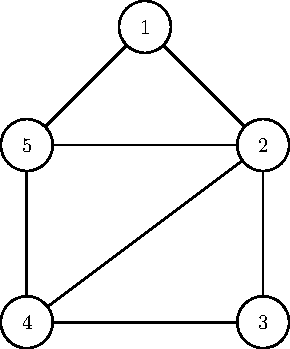
\includegraphics[scale=1]{graphs/graph-coloring-example.pdf}
	\centering
\end{figure}

For this particular graph there are $15$ variables: $x_{ij}$ for all $i \in \{1, \cdots, 5\}$ and for all $j \in \{1, 2, 3\}$. The associated constraints are:

$$ x_{i1} + x_{i2} + x_{i3} = 1 \quad \forall i \in \{1, \cdots, 5\} $$
$$ x_{ic} + x_{jc} \leq 1 \quad \forall c \in \{1, 2, 3\} \quad \text{for all adjacent nodes i and j} $$

a total of $26$: $5$ for assigning one and only one color to each node, and $3$ additional ones per edge in the graph ($7$) for no adjacent equally colored nodes. First, let us rename our variables from $1$ to $15$ as follows:

$$ (x_{11}, x_{12}, x_{13}, x_{21}, x_{22}, x_{23}, x_{31}, \dots, x_{52}, x_{53}) =
	(x_1, x_2, x_3, x_4, x_5, x_6, x_7, \dots, x_{15}, x_{16}) $$

The first set of constraints may be substitued by $P(x_{i1} + x_{i2} + x_{i3} - 1)^2$, which only equals $0$ if the constraint is satisfied. For instance, for the first node $P(x_1 + x_2 + x_3 - 1)^2$ is tranformed to $P(- x_1 - x_2 - x_3 + 2 x_1 x_2 + 2 x_1 x_3 + 2 x_2 x_3 + 1)$. By chosing a value for $P=4$ and dropping the constant we can  insert these penalties into an under developed $Q$ matrix:

$$
Q = 
\left(
\begin{array}{*{15}c}
	-4 & 4 & 4 & 0 & 0 & 0 & 0 & 0 & 0 & 0 & 0 & 0 & 0 & 0 & 0 \\
	4 & -4 & 4 & 0 & 0 & 0 & 0 & 0 & 0 & 0 & 0 & 0 & 0 & 0 & 0 \\
	4 & 4 & -4 & 0 & 0 & 0 & 0 & 0 & 0 & 0 & 0 & 0 & 0 & 0 & 0 \\
	0 & 0 & 0 & -4 & 4 & 4 & 0 & 0 & 0 & 0 & 0 & 0 & 0 & 0 & 0 \\
	0 & 0 & 0 & 4 & -4 & 4 & 0 & 0 & 0 & 0 & 0 & 0 & 0 & 0 & 0 \\
	0 & 0 & 0 & 4 & 4 & -4 & 0 & 0 & 0 & 0 & 0 & 0 & 0 & 0 & 0 \\
	0 & 0 & 0 & 0 & 0 & 0 & -4 & 4 & 4 & 0 & 0 & 0 & 0 & 0 & 0 \\
	0 & 0 & 0 & 0 & 0 & 0 & 4 & -4 & 4 & 0 & 0 & 0 & 0 & 0 & 0 \\
	0 & 0 & 0 & 0 & 0 & 0 & 4 & 4 & -4 & 0 & 0 & 0 & 0 & 0 & 0 \\
	0 & 0 & 0 & 0 & 0 & 0 & 0 & 0 & 0 & -4 & 4 & 4 & 0 & 0 & 0 \\
	0 & 0 & 0 & 0 & 0 & 0 & 0 & 0 & 0 & 4 & -4 & 4 & 0 & 0 & 0 \\
	0 & 0 & 0 & 0 & 0 & 0 & 0 & 0 & 0 & 4 & 4 & -4 & 0 & 0 & 0 \\
	0 & 0 & 0 & 0 & 0 & 0 & 0 & 0 & 0 & 0 & 0 & 0 & -4 & 4 & 4 \\
	0 & 0 & 0 & 0 & 0 & 0 & 0 & 0 & 0 & 0 & 0 & 0 & 4 & -4 & 4 \\
	0 & 0 & 0 & 0 & 0 & 0 & 0 & 0 & 0 & 0 & 0 & 0 & 4 & 4 & -4 
\end{array}
\right)
$$

Secondly, in order to transform $x + y \leq 1$ we can refer to table \ref{tab:penalties-table} and use $P(xy)$. We add these penalties to the previous matrix in the proper places:

$$
Q = 
\left(
\begin{array}{*{15}c}
	-4 & 4 & 4 & 2 & 0 & 0 & 0 & 0 & 0 & 0 & 0 & 0 & 2 & 0 & 0 \\
	4 & -4 & 4 & 0 & 2 & 0 & 0 & 0 & 0 & 0 & 0 & 0 & 0 & 2 & 0 \\
	4 & 4 & -4 & 0 & 0 & 2 & 0 & 0 & 0 & 0 & 0 & 0 & 0 & 0 & 2 \\
	2 & 0 & 0 & -4 & 4 & 4 & 2 & 0 & 0 & 2 & 0 & 0 & 2 & 0 & 0 \\
	0 & 2 & 0 & 4 & -4 & 4 & 0 & 2 & 0 & 0 & 2 & 0 & 0 & 2 & 0 \\
	0 & 0 & 2 & 4 & 4 & -4 & 0 & 0 & 2 & 0 & 0 & 2 & 0 & 0 & 2 \\
	0 & 0 & 0 & 2 & 0 & 0 & -4 & 4 & 4 & 2 & 0 & 0 & 0 & 0 & 0 \\
	0 & 0 & 0 & 0 & 2 & 0 & 4 & -4 & 4 & 0 & 2 & 0 & 0 & 0 & 0 \\
	0 & 0 & 0 & 0 & 0 & 2 & 4 & 4 & -4 & 0 & 0 & 2 & 0 & 0 & 0 \\
	0 & 0 & 0 & 2 & 0 & 0 & 2 & 0 & 0 & -4 & 4 & 4 & 2 & 0 & 0 \\
	0 & 0 & 0 & 0 & 2 & 0 & 0 & 2 & 0 & 4 & -4 & 4 & 0 & 2 & 0 \\
	0 & 0 & 0 & 0 & 0 & 2 & 0 & 0 & 2 & 4 & 4 & -4 & 0 & 0 & 2 \\
	2 & 0 & 0 & 2 & 0 & 0 & 0 & 0 & 0 & 2 & 0 & 0 & -4 & 4 & 4 \\
	0 & 2 & 0 & 0 & 2 & 0 & 0 & 0 & 0 & 0 & 2 & 0 & 4 & -4 & 4 \\
	0 & 0 & 2 & 0 & 0 & 2 & 0 & 0 & 0 & 0 & 0 & 2 & 4 & 4 & -4 
\end{array}
\right)
$$

Since the matrix above incorporates all the constraints, finding a graph coloring is equivalent to finding a minimum of:

$$ \text{Minimize } f(x) = x^T Q x $$

Solving this model using quantum annealing yields a possible solution: $x_2 = x_4 = x_9 = x_{11} = x_{15} = 1$, and $0$ for the rest of the variables. Meaning, nodes $1$ and $4$ are assigned color number $2$, node $2$ is assigned color number $1$, and nodes $3$ and $5$ are assigned color number $3$.

As a final remark, this method of graph coloring has proven to be computationally useful for graphs with up to $450$ nodes and $9757$ edges \cite{Kochenberger2005}.


\subsection{The Travelling Salesman problem}
\label{sec:tsp-qubo}


This example is mainly based on \cite{Glover2019}.

In order to formulate our next problem, a couple of extra definitions are needed. Given a graph, a \emph{Hamiltonian path} is a path -a sequence of connected nodes- such that it only passes through each node exactly once. A \emph{cycle}, also called \emph{tour}, is a path that starts and ends in the same node. A \emph{Hamiltonian cycle} is a cycle that passes through each node a single time, except for the first/last node which appears twice in the cycle. Additionally, a weighted graph $G =(V, E, W)$ is a graph with a series of weights $w_e \in \R$, each associated to an edge $e \in E$.

The Travelling Salesman problem is the following: Given a directed weighted graph, find a Hamiltonian cycle with minimum total weight. The problem is sometimes stated with a Hamiltonian path instead of a Hamiltonian cycle, but as it will be seen in section [TODOref], for our purposes the cycle-statement will be of better use.

We may suppose without losing generality that the graph is complete. That is, there is always an edge from every two nodes in every direction. If the given graph is not complete, we may add the remaining edges with a high enough weight so that they are never used.

Since solutions to this problem are a series of $n \equiv |V|$ nodes -the number of nodes in the graph-, we will encode $n$-nodes cycles as $(v_{k_0}, \ldots, v_{k_{n-1}})$, where nodes $v_{k_0}$ and $v_{k_{n-1}}$ are also conected. Thus, our problem may originally may stated as:

$$ \text{Minimize } \sum_{i=0}^{n-1} w_{k_i, k_{i+1}} $$
$$ \text{subject to the constraint that } (v_{k_0}, \cdots, v_{k_{n-1}}) \text{ e}$$

where $w_{k_i, k_{i+1}}$ is the weight associated to the edge connecting nodes $v_{k_i}$ and $v_{k_{i+1}}$; and where the addition is performed under modulus $n$: $k_n \equiv k_0$. The binary variables $x_{i,p}$ will be used, where $i,p \in \{0, \ldots, n-1\}$. $x_{i,p}$ will equal $1$ if and only if node $i$ is in position $p$ in our cycle. Hence, we will have $n^2$ variables under the following constraints:

\begin{enumerate}
	\item Every node must be assigned. Thus, node assigment will be rewarded with a non-positive weight (favorable bias) called \textbf{self-bias} with an associated non-positive penalty:
	
	$$ a x_{i,p} \quad \forall i,p \in \{0, \ldots, n-1\} $$
	
	where $a \leq 0$. In practice, this will not be necessary for every problem. We may remove the self-bias by setting $a=0$. Adding these penalties for every node and position yields:
	
	\begin{equation}
		\label{eqn:salesman-constrain1}
		a \sum_{i=0}^{n-1} \sum_{p=0}^{n-1} x_{i,p}
	\end{equation}
	
	\item Every node must be assigned to only one position. This constraint will be called \textbf{repetition}:
	
	$$ \sum_{p=0}^{n-1} x_{i,p} = 1 \quad \forall p \in \{0, \ldots, n-1\} $$
	
	Resulting in the following penalty:
	
	$$ b \Big( \sum_{p=0}^{n-1} x_{i,p} - 1 \Big)^2 \quad \forall p \in \{0, \ldots, n-1\} $$

	where $b$ is a positive parameter. Adding these penalties for eveyr node we obtain:
	
	\begin{equation}
		\label{eqn:salesman-constrain2}
		b \sum_{i=0}^{n-1} \Big( \sum_{p=0}^{n-1} x_{i,p} - 1 \Big)^2
	\end{equation}
		
	\item Every position must be assigned only one node. This constraint will be called \textbf{colocation}:
	
	$$ \sum_{i=0}^{n-1} x_{i,p} = 1 \quad \forall i \in \{0, \ldots, n-1\} $$
	
	Resulting in the following total penalty:
	
	\begin{equation}
		\label{eqn:salesman-constrain3}
		c \sum_{p=0}^{n-1} \Big( \sum_{i=0}^{n-1} x_{i,p} - 1 \Big)^2
	\end{equation}
	
	where $c$ is a positive parameter.	
\end{enumerate}

Finally, we may re-write the cost function in terms of the binary variables. Weight $w_{ij}$ must be added in the cost function if and only if nodes $i$ and $j$ follow each other in the path. That is, if and only if $x_{i,p}x_{j,p+1} = 1$ for any position $p$. In fact, it may be needed to add it multiple times if the previous equality holds for multiple positions. Thus, the penalty associated to weight $w_{i,j}$ is:

$$ w_{i,j} \sum_{p=0}^{n-1} x_{i,p}x_{j,p+1} $$

Adding up the penalties associated with every weight yields the cost function:

$$ \text{Minimize } \sum_{i=0}^{n-1} \sum_{j=0}^{n-1} w_{i,j}\sum_{p=0}^{n-1} x_{i,p}x_{j,p+1} $$

The final QUBO model is obtained by adding the penalties \ref{eqn:salesman-constrain1}, \ref{eqn:salesman-constrain2} and \ref{eqn:salesman-constrain3} to the cost function:

% Using an extra column for left aligment.
\begin{equation}
	\begin{alignedat}{3}
		& \text{Minimize }	&& \sum_{i=0}^{n-1} \sum_{j=0}^{n-1} w_{i,j}\sum_{p=0}^{n-1} x_{i,p}x_{j,p+1} & \\
		& && + a \sum_{i=0}^{n-1} \sum_{p=0}^{n-1} x_{i,p} & \qquad \text{(self-bias)} \\
		& && + b \sum_{i=0}^{n-1} \Big( \sum_{p=0}^{n-1} x_{i,p} - 1 \Big)^2 & \qquad \text{(repetition)} \\
		& && + c \sum_{p=0}^{n-1} \Big( \sum_{i=0}^{n-1} x_{i,p} - 1 \Big)^2 & \qquad \text{(colocation)}
	\end{alignedat}
	\label{eqn:salesman-cost-funct}
\end{equation}


Since this is a quadratic unconstraint function, this is already a QUBO. The conversion to a matrix is straightforward. Let us see this in an example.


\newparagraph{Numerical Example}
\label{sec:salesman-example}


Given the following graph:

\begin{figure}[H]
	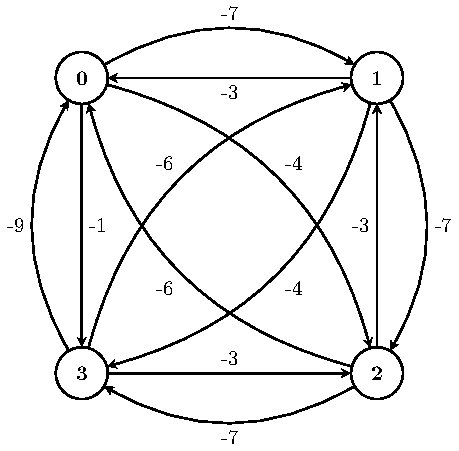
\includegraphics[scale=1.1]{graphs/salesman-example.pdf}
	\centering
	\label{fig:salesman-graph} % used in chapter 3
\end{figure}

Find a Hamiltonian cycle with minimum c\begin{table}[H]
	\centering
	\makebox[\textwidth][c]{
		\begin{tabular}{ccc}		
			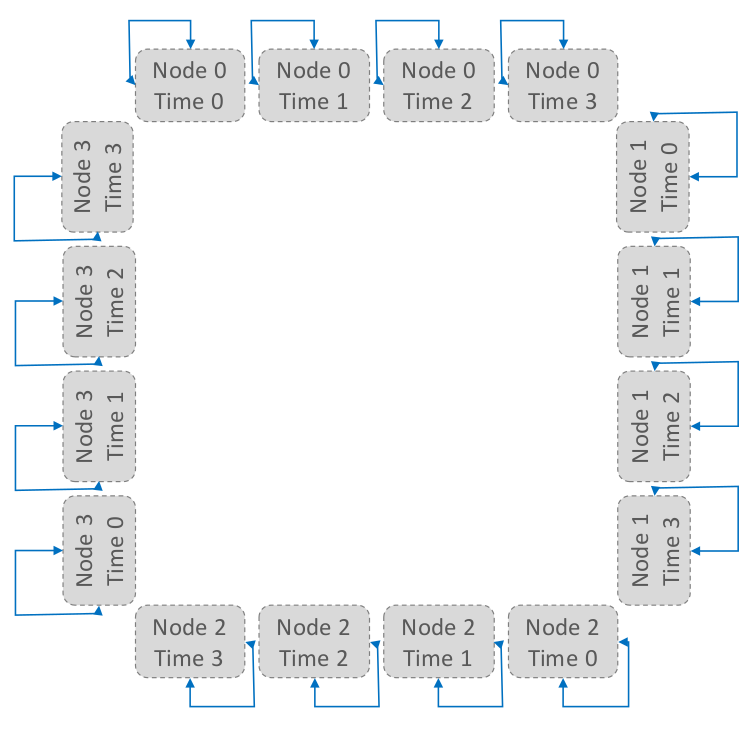
\includegraphics[scale=0.2]{salesman-penalties1.png} &
			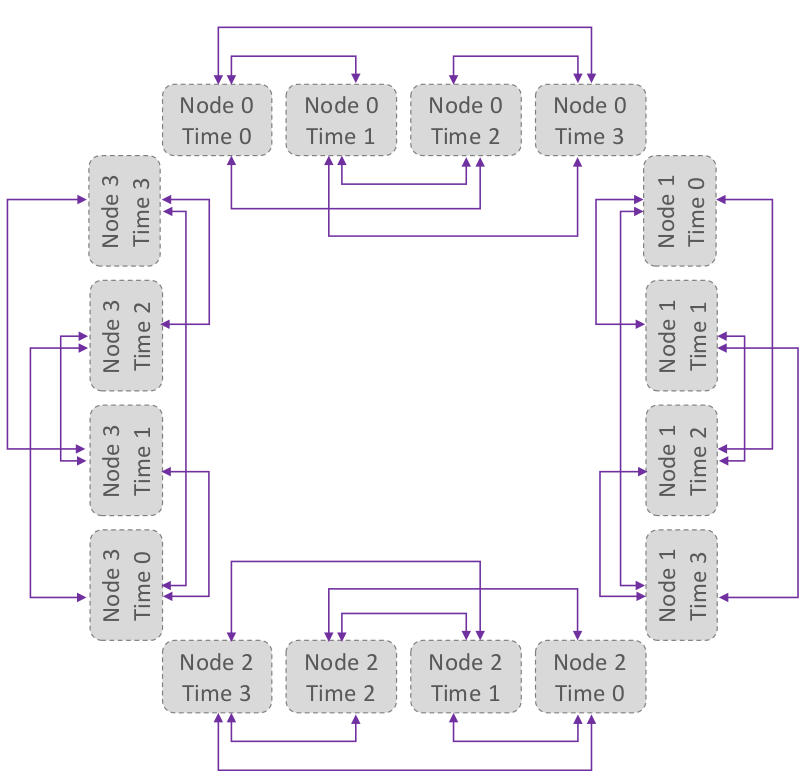
\includegraphics[scale=0.2]{salesman-penalties2.png} &
			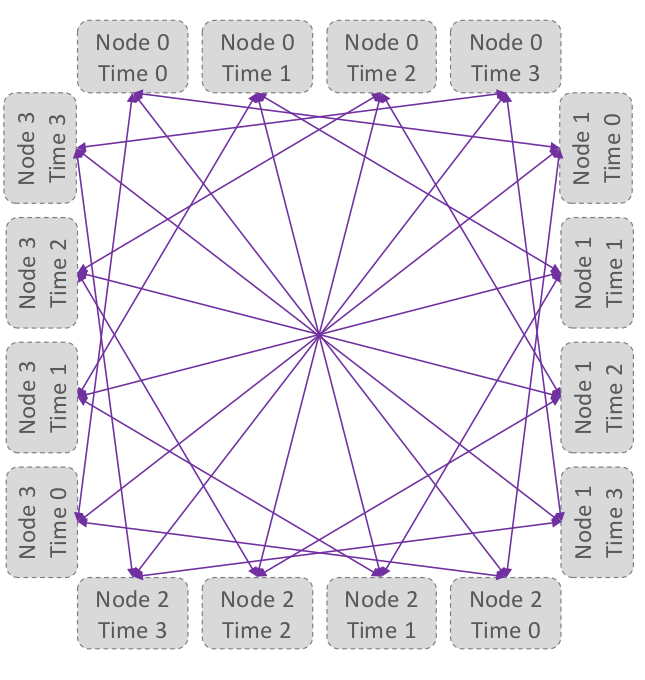
\includegraphics[scale=0.2]{salesman-penalties3.png} \\
			
			1: Self-bias & 2: Repetition & 3: Colocation \\
			
			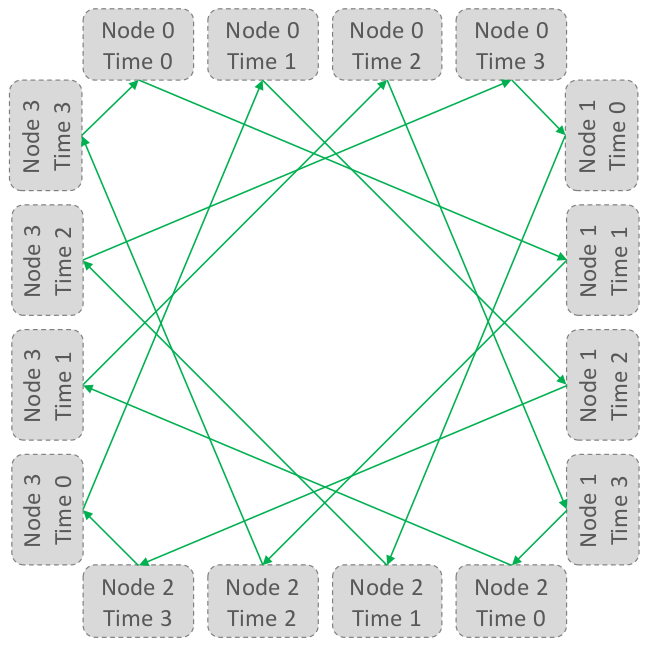
\includegraphics[scale=0.2]{salesman-penalties4.png} &
			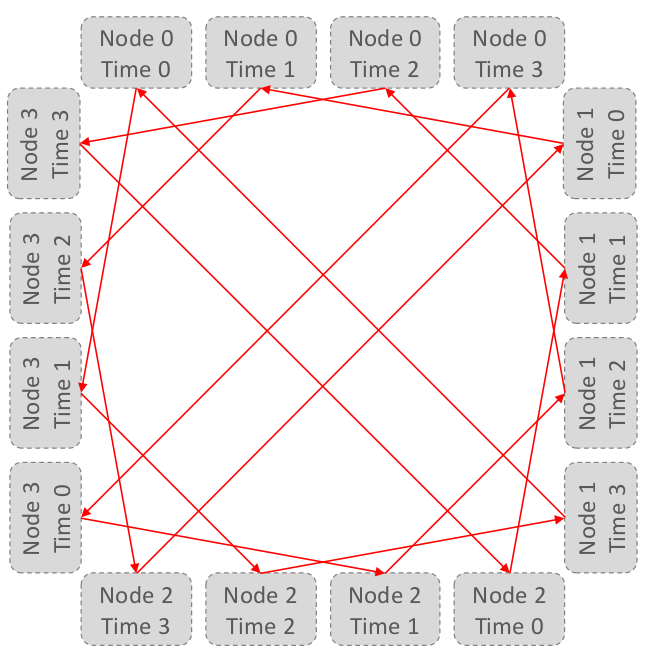
\includegraphics[scale=0.2]{salesman-penalties5.png} &
			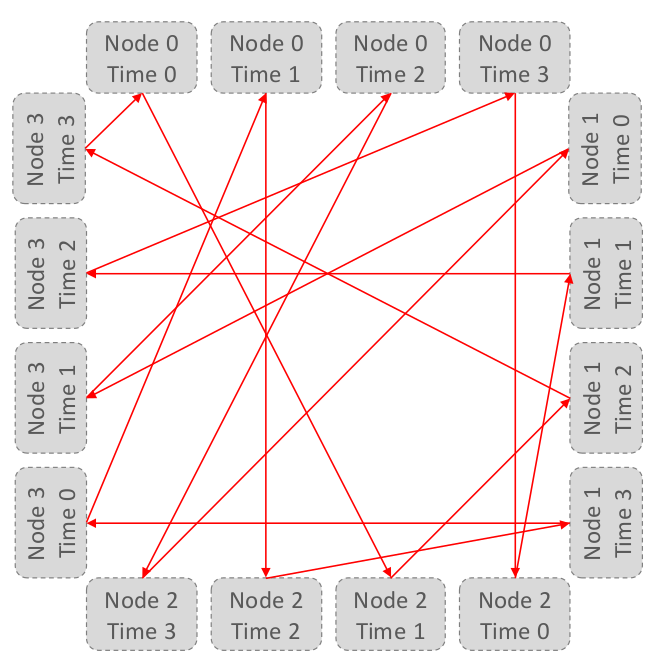
\includegraphics[scale=0.2]{salesman-penalties6.png} \\
			
			4: Type A tours & 5: Type B tours & 6: Type C tours \\
			
			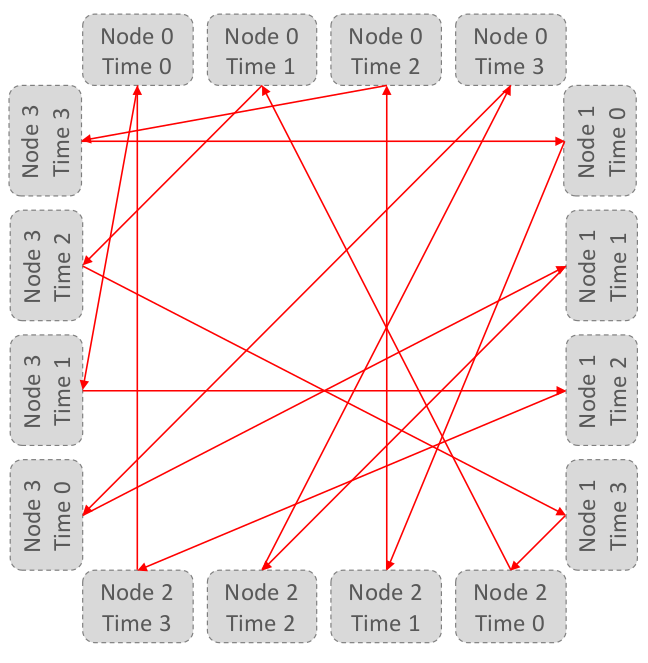
\includegraphics[scale=0.2]{salesman-penalties7.png} &
			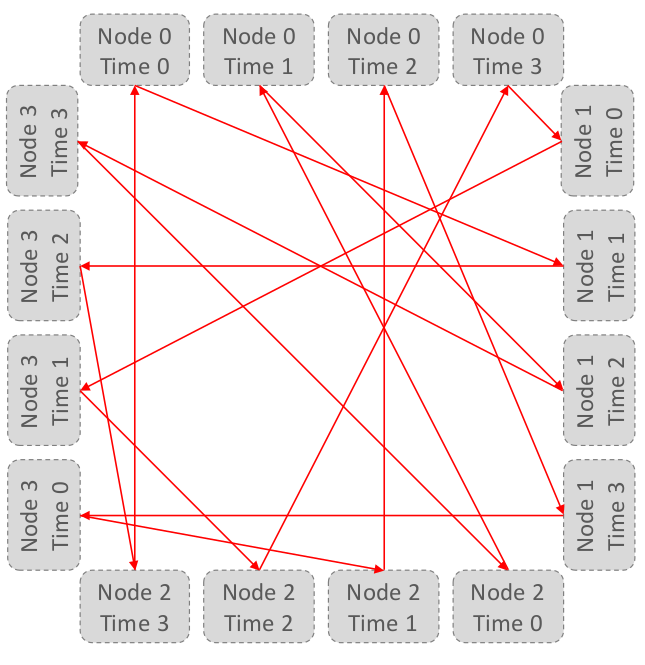
\includegraphics[scale=0.2]{salesman-penalties8.png} &
			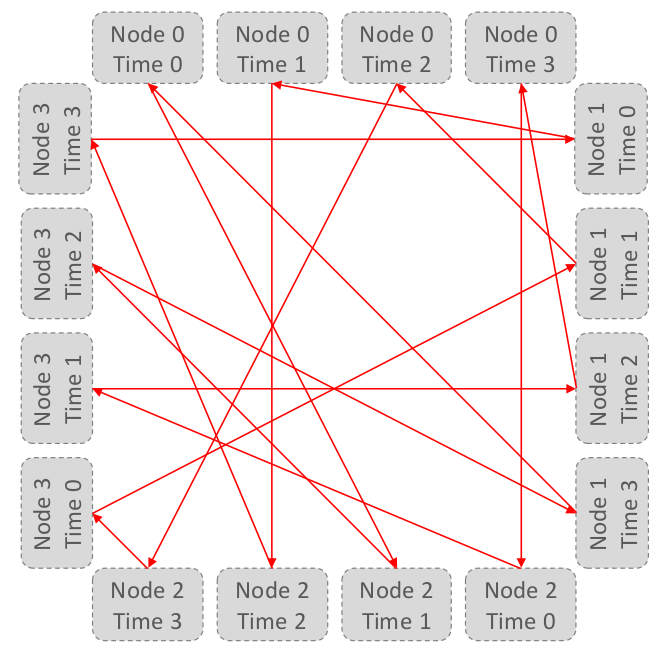
\includegraphics[scale=0.2]{salesman-penalties9.png} \\
			
			7: Type D tours & 8: Type E tours & 9: Type F tours \\
		\end{tabular}
	}
	\caption{Graphical representation of penalties between interactions \cite{Sarkar2020}}
	\label{fig:salesman-penalties}
\end{table}ost. 

First of all, let us take a deeper look into our possible solutions. There are $(n-1)!$ cycles in a graph with $n$ nodes. For our $4$-nodes graph there are $3! = 6$ type of cycles:

\begin{itemize}
	\item Type A: $0 \rightarrow 1 \rightarrow 2 \rightarrow 3 \rightarrow 0$
	\item Type B: $0 \rightarrow 3 \rightarrow 2 \rightarrow 1 \rightarrow 0$
	\item Type C: $0 \rightarrow 2 \rightarrow 1 \rightarrow 3 \rightarrow 0$
	\item Type D: $0 \rightarrow 3 \rightarrow 1 \rightarrow 2 \rightarrow 0$
	\item Type E: $0 \rightarrow 1 \rightarrow 3 \rightarrow 2 \rightarrow 0$
	\item Type F: $0 \rightarrow 2 \rightarrow 3 \rightarrow 1 \rightarrow 0$
\end{itemize}

We may see this graphically in table \ref{tbl:salesman-cycles}.

\begin{table}[H]
	\centering
	\begin{tabular}{ccc}		
		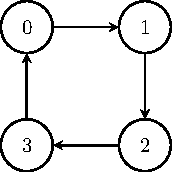
\includegraphics[scale=.9]{graphs/salesman-cycleA.pdf} &
		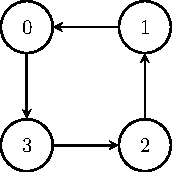
\includegraphics[scale=.9]{graphs/salesman-cycleB.pdf} &
		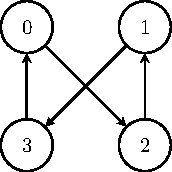
\includegraphics[scale=.9]{graphs/salesman-cycleC.pdf} \\
		
		Type A & Type B & Type C \\
		
		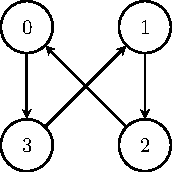
\includegraphics[scale=.9]{graphs/salesman-cycleD.pdf} &
		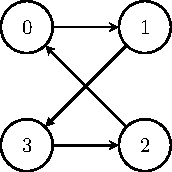
\includegraphics[scale=.9]{graphs/salesman-cycleE.pdf} &
		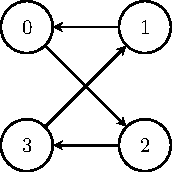
\includegraphics[scale=.9]{graphs/salesman-cycleF.pdf} \\
		
		Type D & Type E & Type F \\
	\end{tabular}
	\caption{Type of cycles in a $4$-nodes graph}
	\label{tbl:salesman-cycles}
\end{table}

These six are the only possible cycles through our graph and one of them will have minimum cost. Since our binary encoding additionally depends on the node position, there are $4$ solutions of our encoding that represent the same cycle. For example, ($0 \rightarrow 1 \rightarrow 2 \rightarrow 3 \rightarrow 0$) and ($1 \rightarrow 2 \rightarrow 3 \rightarrow 0 \rightarrow 1$) both represent cycle type A. In this case, type A will be the tour with minimum cost.

A graphical representation of the different penalties interactions is shown in figure \ref{fig:salesman-penalties}, based on the constraints defined above.

\begin{table}[H]
	\centering
	\makebox[\textwidth][c]{
		\begin{tabular}{ccc}		
			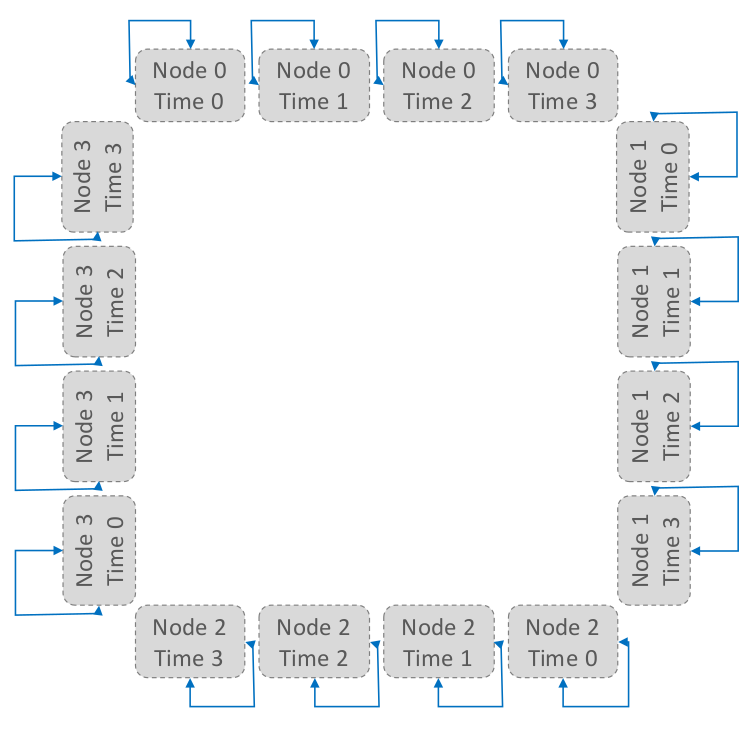
\includegraphics[scale=0.2]{salesman-penalties1.png} &
			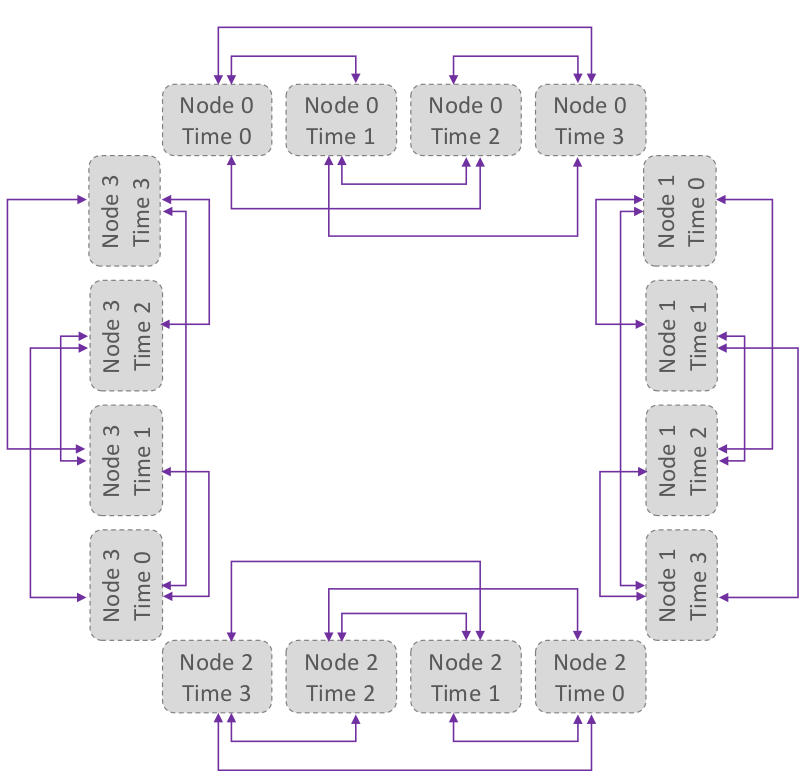
\includegraphics[scale=0.2]{salesman-penalties2.png} &
			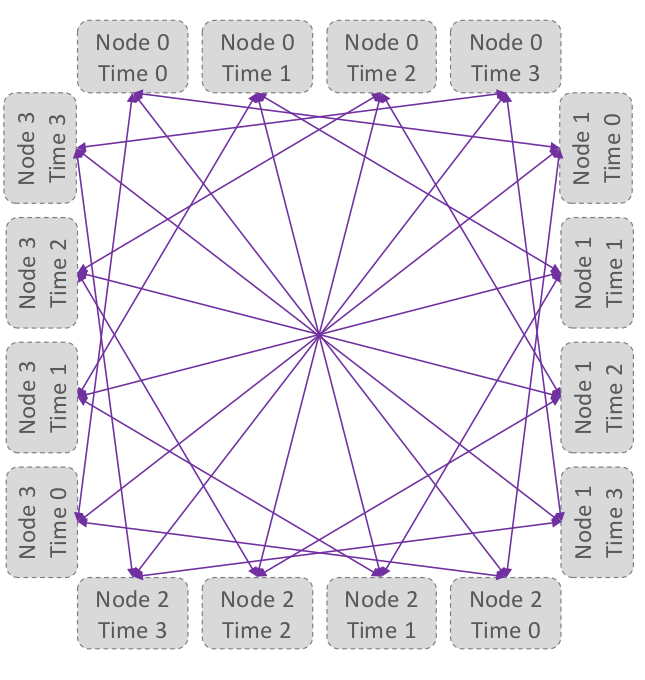
\includegraphics[scale=0.2]{salesman-penalties3.png} \\
			
			1: Self-bias & 2: Repetition & 3: Colocation \\
			
			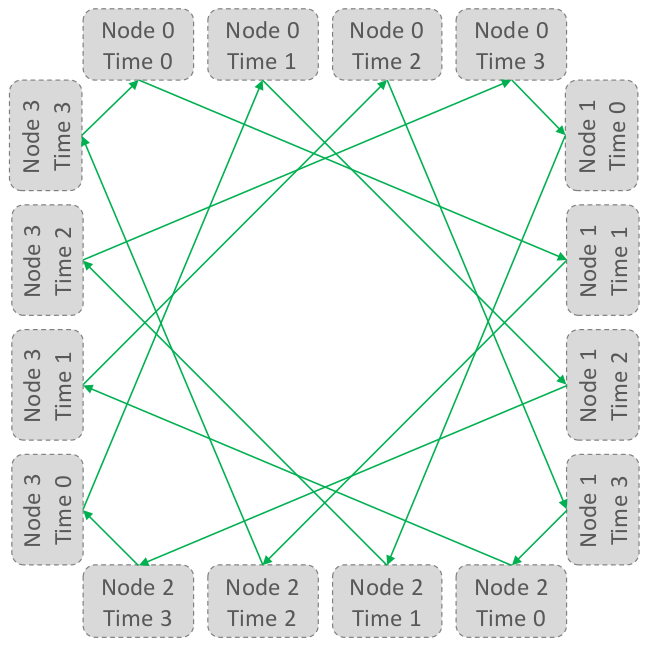
\includegraphics[scale=0.2]{salesman-penalties4.png} &
			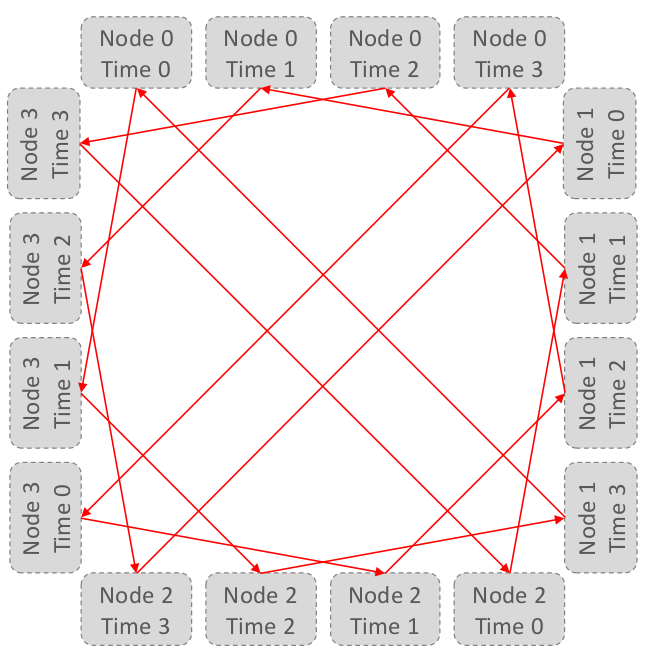
\includegraphics[scale=0.2]{salesman-penalties5.png} &
			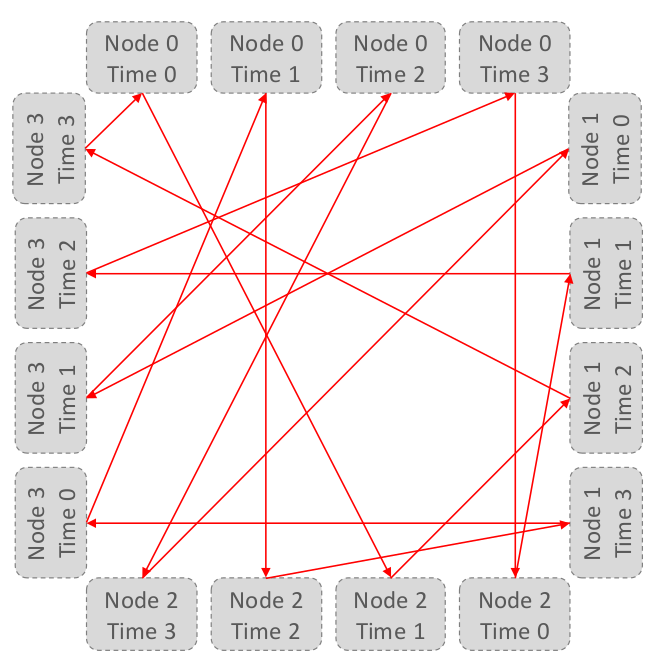
\includegraphics[scale=0.2]{salesman-penalties6.png} \\
			
			4: Type A tours & 5: Type B tours & 6: Type C tours \\
			
			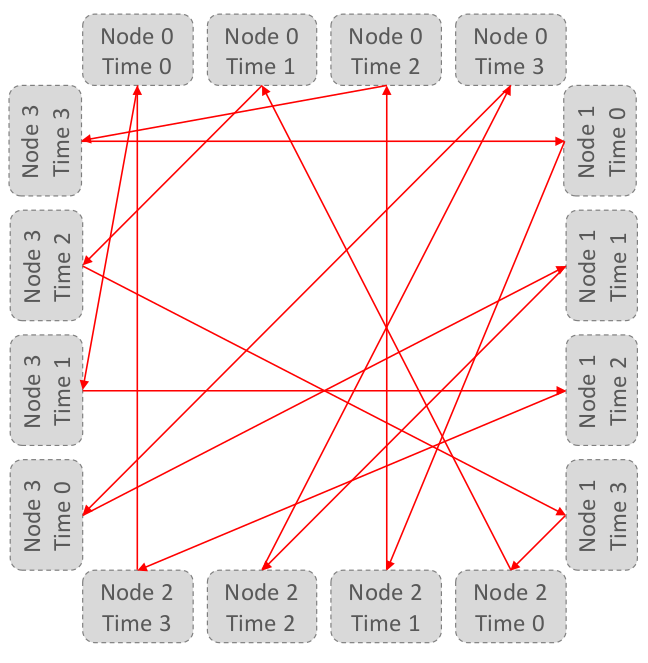
\includegraphics[scale=0.2]{salesman-penalties7.png} &
			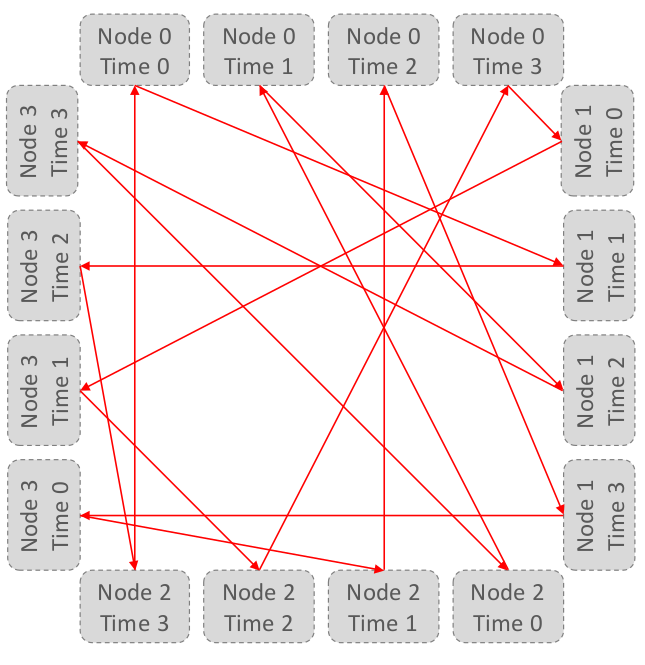
\includegraphics[scale=0.2]{salesman-penalties8.png} &
			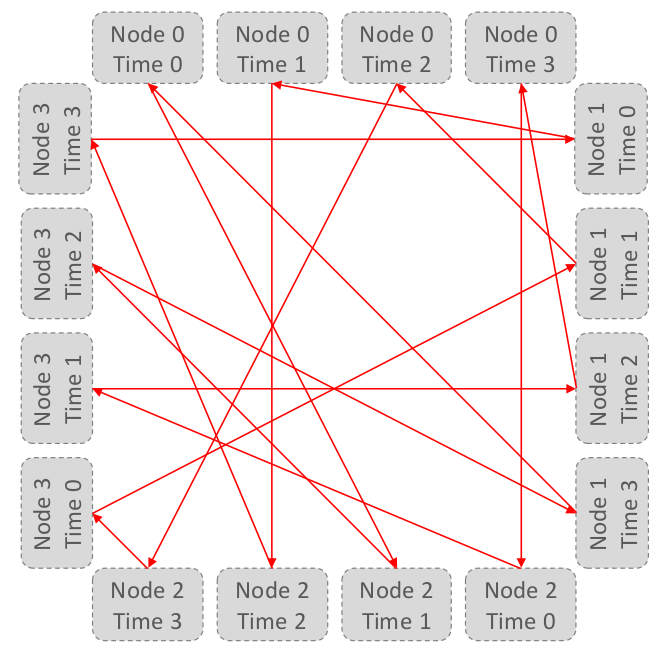
\includegraphics[scale=0.2]{salesman-penalties9.png} \\
			
			7: Type D tours & 8: Type E tours & 9: Type F tours \\
		\end{tabular}
	}
	\caption{Graphical representation of penalties between interactions \cite{Sarkar2020}}
	\label{fig:salesman-penalties}
\end{table}

We start the problem refactoring by renaming the variables:

$$ (x_{0,0}, x_{0,1}, x_{0,2}, x_{0,3}, x_{1,0}, x_{1,1}, x_{1,2}, \dots, x_{3,2}, x_{3,3}) =
(x_1, x_2, x_3, x_4, x_5, x_6, x_7, \dots, x_{15}, x_{16}) $$

\begin{figure}[H]
	\makebox[\textwidth][c]{
		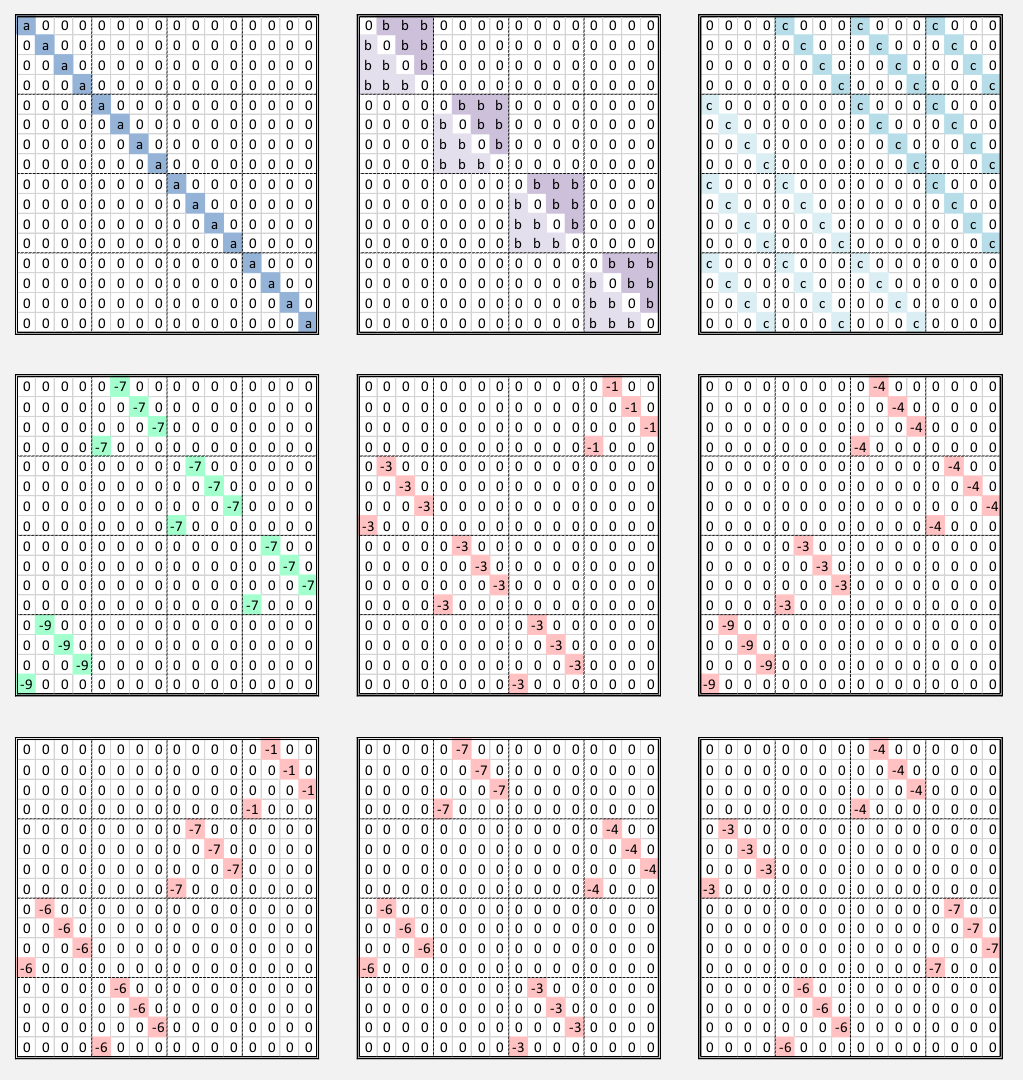
\includegraphics[scale=0.5]{salesman-adj-matrices.png}
	}
	\centering
	\caption{Term by term penalty matrices \cite{Sarkar2020}}
	\label{fig:salesman-adj-matrices}
\end{figure}

Each of the terms in the cost function \ref{eqn:salesman-cost-funct} may be transformed into a matrix. The term associated to the weights is additionally split using the different types of cycles in which they appear. We thus obtain nine adjacency matrices, found on figure \ref{fig:salesman-adj-matrices}.

Note that the matrices associated with the constraints are all symmetric. This happens because they only depend on the graph topology and not on the weights. On the other hand, since the cost of going back and forth between a pair of nodes is not the same, the matrices associated with the cycles are never symmetric.

The final $Q$ matrix for our problem is obtained by adding these matrices. Experimental evidence suggests that setting $a = 0$ and $b = c = 13$, and applying quantum annealing yields optimal solutions for our cost function \cite{Sarkar2020}. Using these values for the penalties, the final $Q$ matrix is seen in figure \ref{fig:salesman-Q-matrix}.

\begin{figure}[H]
	\makebox[\textwidth][c]{
		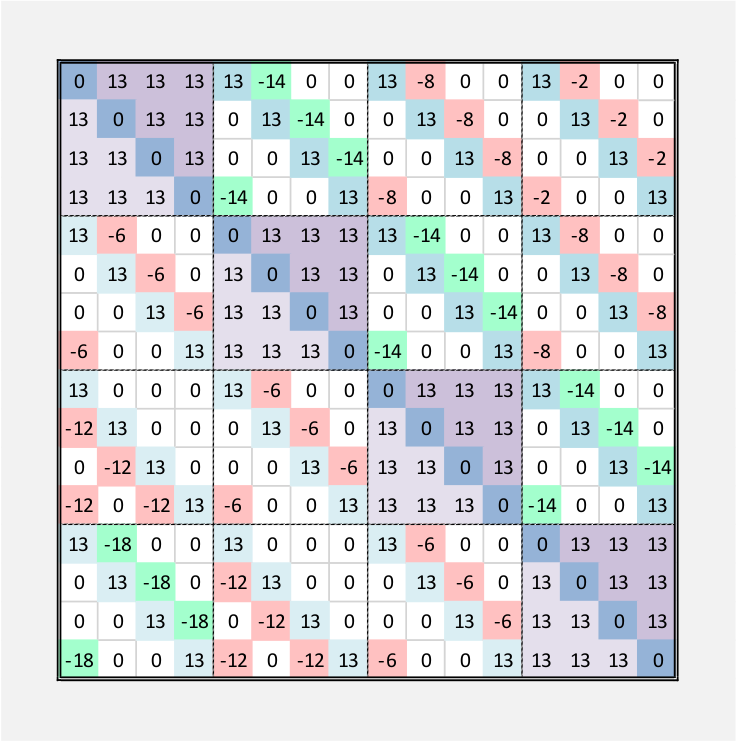
\includegraphics[scale=0.4]{salesman-Q-matrix.png}
	}
	\centering
	\caption{Final Q-matrix \cite{Sarkar2020}}
	\label{fig:salesman-Q-matrix}
\end{figure}

Finally transforming our problem into a QUBO in its matrix form, using the previous matrix:

$$ \text{Minimize } f(x) = x^T Q x $$

Finding one of the following minimas:

\begin{itemize}
	\item $x^T = [1000010000100001]$, equivalent to $x_{0,0} = x_{1,1} = x_{2,2} = x_{3,3} = 1$ and $0$ otherwise. Or in path notation: $(0 \rightarrow 1 \rightarrow 2 \rightarrow 3 \rightarrow 0)$
	\item $x^T = [0100001000011000]$, equivalent to $x_{0,1} = x_{1,2} = x_{2,3} = x_{3,0} = 1$ and $0$ otherwise. Or in path notation: $(1 \rightarrow 2 \rightarrow 3 \rightarrow 0 \rightarrow 1)$
	\item $x^T = [0010000110000100]$, equivalent to $x_{0,2} = x_{1,3} = x_{2,0} = x_{3,1} = 1$ and $0$ otherwise. Or in path notation: $(2 \rightarrow 3 \rightarrow 0 \rightarrow 1 \rightarrow 2)$
	\item $x^T = [0001100001000010]$, equivalent to $x_{0,3} = x_{1,0} = x_{2,1} = x_{3,2} = 1$ and $0$ otherwise. Or in path notation: $(3 \rightarrow 0 \rightarrow 1 \rightarrow 2 \rightarrow 3)$
\end{itemize}

Which corresponds to the four ways of encoding type A cycles with our notation.


\FloatBarrier
\section{D-Wave Systems}
\label{sec:d-wave-systems}


\textbf{D-Wave Systems Inc.} is a Canadian company dedicated to quantum computing. In 2011, they announced the first commercial quantum computer system, D-Wave One. During the following two decades, the D-Wave team has developed a series of quantum computers dedicated to quantum annealing. The last one being the Advantage System (figure \ref{fig:advantage}).

\begin{figure}[h]
	\includegraphics[scale=.1]{advantage_system.png}
	\centering
	\caption{Advantage$^{TM}$ system}
	\label{fig:advantage}
\end{figure}

The quantum processing unit (QPU) of this system consists of $5640$ qubits and $40,484$ \emph{couplers} (links between qubits that allow entanglement between a pair of qubits). It can be seen in figure \ref{fig:QPU}. The number of couplers is especially relevant. A coupler is a physical mechanism that allows two qubits to be entangled. We will explain couplers in-depth in the next section. The different D-Wave architectures are explained in section \ref{sec:topologies}. In table \ref{tab:dwave-comp}, we see a comparison between the number of qubits and couplers from the different versions of the D-Wave computer system.

\begin{table}[h]
	\centering
	\makebox[\textwidth][c]{
		\begin{tabular}{cccccc}
							& D-Wave One 	& D-Wave Two	& D-Wave 2X 	& D-Wave 2000Q 	& Advantage \\ \hline
			Release date 	& May 2011	 	& May 2013 		& August 2015	& January 2017	& 2020   	\\
			Qubits 			& $128$	 		& $512$ 		& $1152$		& $2048$		& $5640$  	\\
			Couplers 		& $352$	 		& $1,472$ 		& $3,360$		& $6,016$		& $40,484$  
		\end{tabular}
	}
	\caption{D-Wave historical comparison \cite{DwaveWikipedia}}
	\label{tab:dwave-comp}
\end{table}

Since the QPU must be isolated to operate, it is encapsulated in a system at temperatures below 15 mK. In addition, radio frequency (RF)-shielded enclosure and magnetic shieldings are used to protect it from electromagnetic interference \cite{DWaveDoc}.

\begin{figure}[h]
	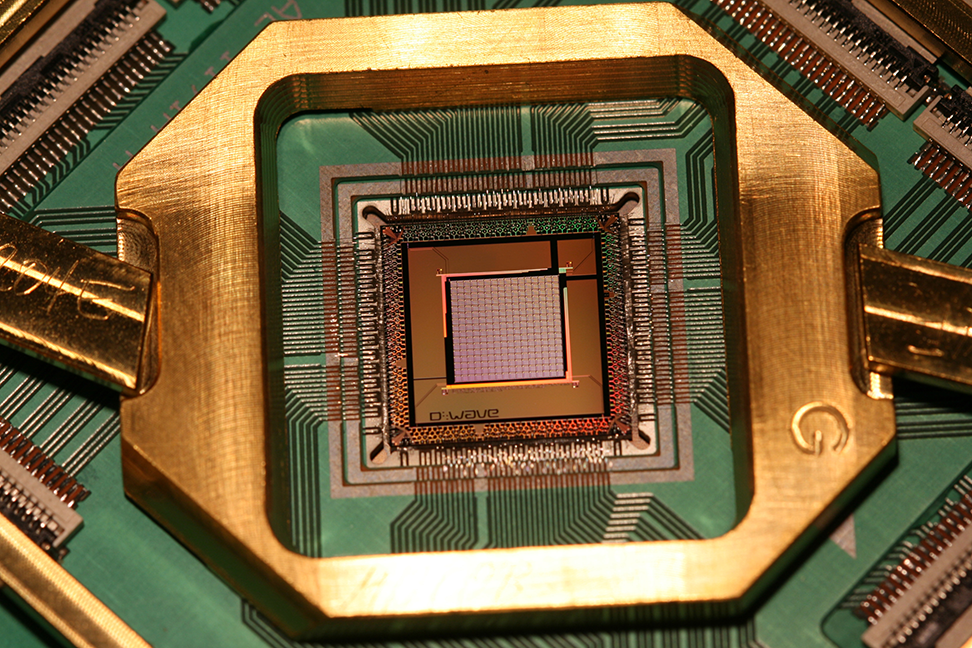
\includegraphics[scale=.2]{qpu.png}
	\centering
	\caption{D-Wave QPU}
	\label{fig:QPU}
\end{figure}

D-Wave provides an easy-to-use software environment to solve problems using quantum annealing. We will explain it in-depth in section [TODOref].


\subsection{Quantum Annealing in D-Wave}
\label{sec:quantum-annealing-dwave}


For this section, we refer to the D-Wave documentation, which explains how quantum annealing is implemented and may be exploited in the D-Wave systems \cite{DWaveDoc-QuantumAnnealing}.

Let us start by describing how qubits are physically implemented in D-Wave's QPU. Superconducting loops are used for this purpose, with a circulating current and a magnetic field. Depending on the direction of the current, the qubit will be in state $0$ or $1$; see figure \ref{fig:dwave-qubit}.

\begin{figure}[h]
	\makebox[\textwidth][c]{
		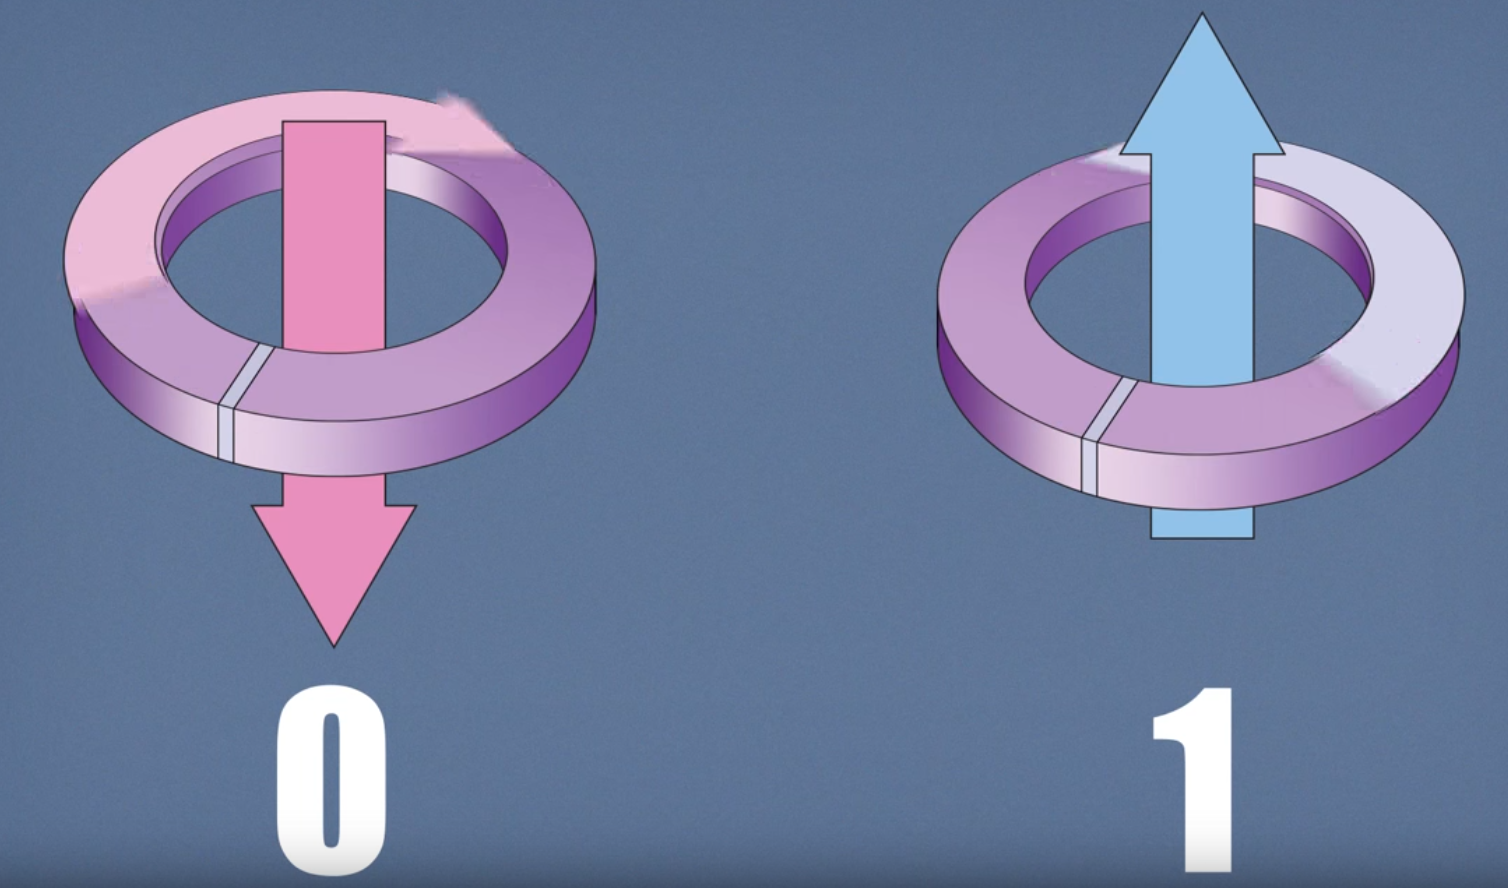
\includegraphics[scale=.2]{dwave-qubit.png}
	}
	\centering
	\caption{D-Wave's qubit, using a circulating current \cite{DWaveDoc-QuantumAnnealing}}
	\label{fig:dwave-qubit}
\end{figure}

In figure \ref{fig:dwave-annealing} we see a diagram with the evolution of a single qubit's energy during the annealing. By applying a magnetic field to the qubit we may affect the current and put the qubit in a superposition of both states (a). At this point, the energy is represented by a single valley with a single minimum: the superposition state where the qubit starts. Remember that at the end of the annealing we will measure every qubit and make them collapse to either one of those states, so we will never see a superposition in our measurements.

\begin{figure}[h]
	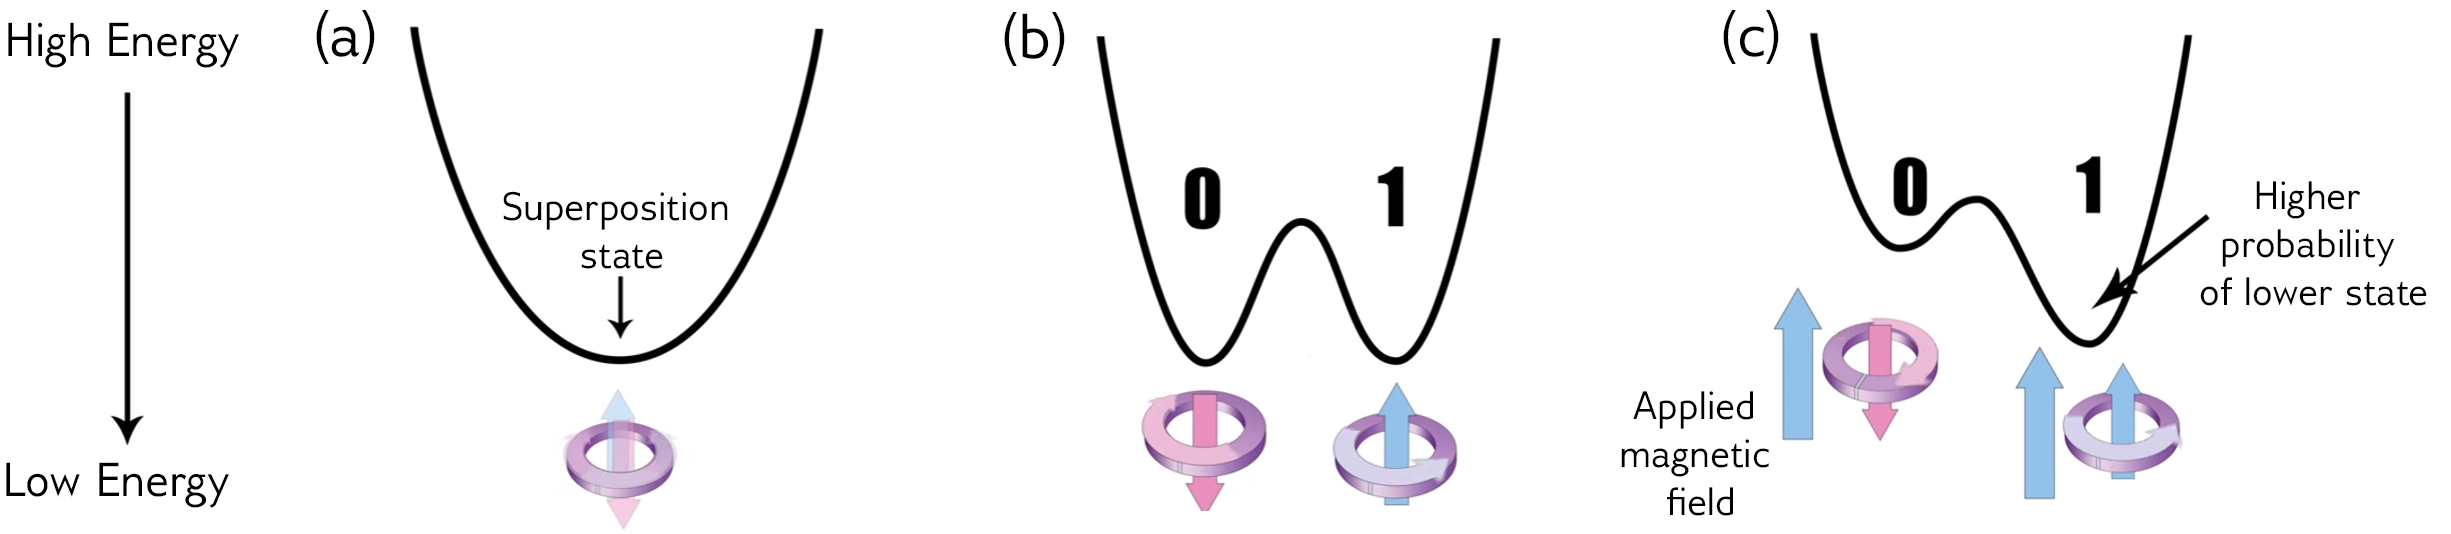
\includegraphics[scale=.2]{dwave-annealing.png}
	\centering
	\caption{Energy diagram changes upon running the annealing and applying bias \cite{DWaveDoc-QuantumAnnealing}}
	\label{fig:dwave-annealing}
\end{figure}

Then, the quantum annealing is run, turning the energy diagram into what is called a \emph{double well potential} (b). The lower point of the left valley corresponds to the $0$ state and the right one to the $1$ state. If we measured the qubit now, it would end up with equal probability in either one of both states. However, we may influence the qubit's energy by applying a magnetic field and tilting the double-well to one of the base states (c), increasing the probability of ending in that state. This new magnetic field is called \emph{bias} and the qubit minimizes the energy subject to the applied bias.

Biases applied on single qubits alone do not take full advantage of quantum annealing. We will also need \emph{couplers}, devices that entangle qubits to each other. A coupler can make two qubits tend to end in the same state or in opposite states with certain strength. As with bias, the coupler strength, usually called \emph{weight}  may be controlled by the programmer. Together the biases and the weights are the parameters that define a problem in the D-Wave system. As the reader may already imagine, these are the parameters of a QUBO / Ising model that we may define.

Consider a 2-qubits system for the following simple example. There will be three parameters: the 2 qubits biases and the coupler weight between them. As we know, two entangled qubits may be in four possible states: $(0,0)$, $(0,1)$, $(1,0)$ or $(0,0)$. The previous parameters define what is known as the \emph{energy landspace}. Figure \ref{fig:dwave-2qubit-landscape} illustrates this idea. The energy of each state depends on the biases and the single weight.

\begin{figure}[h]
	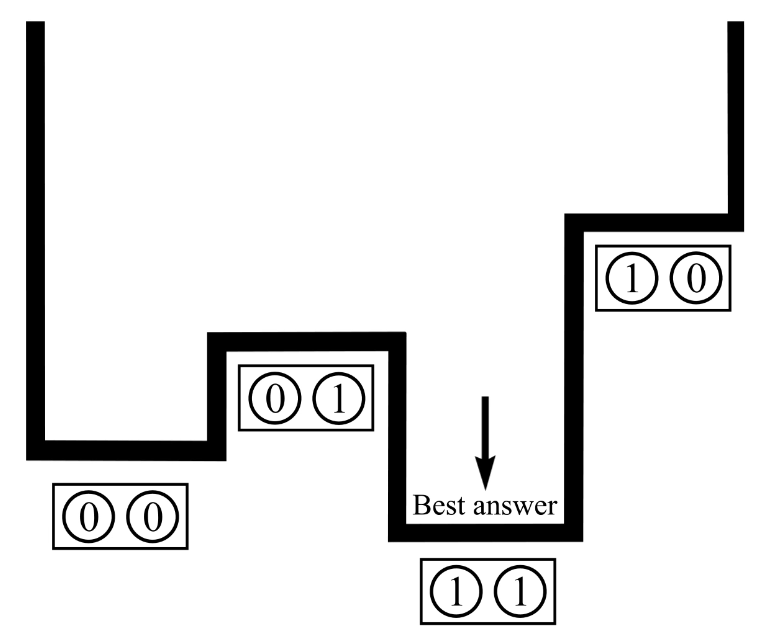
\includegraphics[scale=.25]{dwave-2qubit-landscape.png}
	\centering
	\caption{Example of 2-qubit energy landscape \cite{DWaveDoc-QuantumAnnealing}}
	\label{fig:dwave-2qubit-landscape}
\end{figure}

Let us take a look at the underlying quantum physics of this process. We make use of the Hamiltonian of a quantum system, which describes the evolution of the quantum system as per Postulate 3' [TODOref]. It maps the \emph{eigenstates} of the system to their energies. Only when the system is on an eigenstate, the energy of the system is well defined and called \emph{eigenenergy}, which are just the eigenvalues. The set of eigenstates and eigenenegies is called the \emph{eigenspectrum}. Recall that the lowest energy state is called the \emph{ground state}.

For a D-Wave system, the Hamiltonian may be described as:

$$ H(s) = \underbrace{- \frac{A(s)}{2} \bigg( \sum_i \upsigma_x^{(i)} \bigg)}_\text{Initial Hamiltonian} 
			+ \underbrace{\frac{B(s)}{2} \bigg( \sum_i h_i \upsigma_z^{(i)} + \sum_ {i > j} J_{i,j} \upsigma_z^{(i)} \upsigma_z^{(j)} \bigg)}_\text{Final Hamiltonian} $$

where $\upsigma^{(i)}_{x,z}$ are the Pauli matrices $X$ and $Z$ respectively operating on qubit $(i)$, $h_i$ are the qubit biases, and $J_{i,j}$ are the couplers weights.

As explained in the adiabatic evolution section \ref{sec:adiabatic-evolution}, the Hamiltonian is made of two terms:

\begin{itemize}
	\item The Initial Hamiltonian, also called \emph{tunneling Hamiltonian}, where the ground state is when every qubit is in superposition but no entanglement between qubit takes place.
	\item The Final Hamiltonian, also called \emph{problem Hamiltonian}, where the biases and weights are such that the ground state is the solution of the problem we are trying to solve.
\end{itemize}

In fact, the final Hamiltonian is precisely an Ising model. By expressing our problem as an Ising -or, equivalently, a QUBO- we may encode it inside this Hamiltonian using the parameters $h_i$ and $J_{i,j}$.

We may parametrize $s \in [0,1]$ as an abstract parameter that controls the annealing timing. Assuming the initial time is $t_0 = 0$, $s$ is defined as $s \equiv t / t_{final}$. Thus, the annealing occurs when $s$ goes from $0$ to $1$. We may define the annealing functions $A(s), B(s)$ such that $A(0) \gg B(0)$ and $A(1) \ll B(1)$. For instance, as seen in figure \ref{fig:dwave-annealing-functions}.

\begin{figure}[h]
	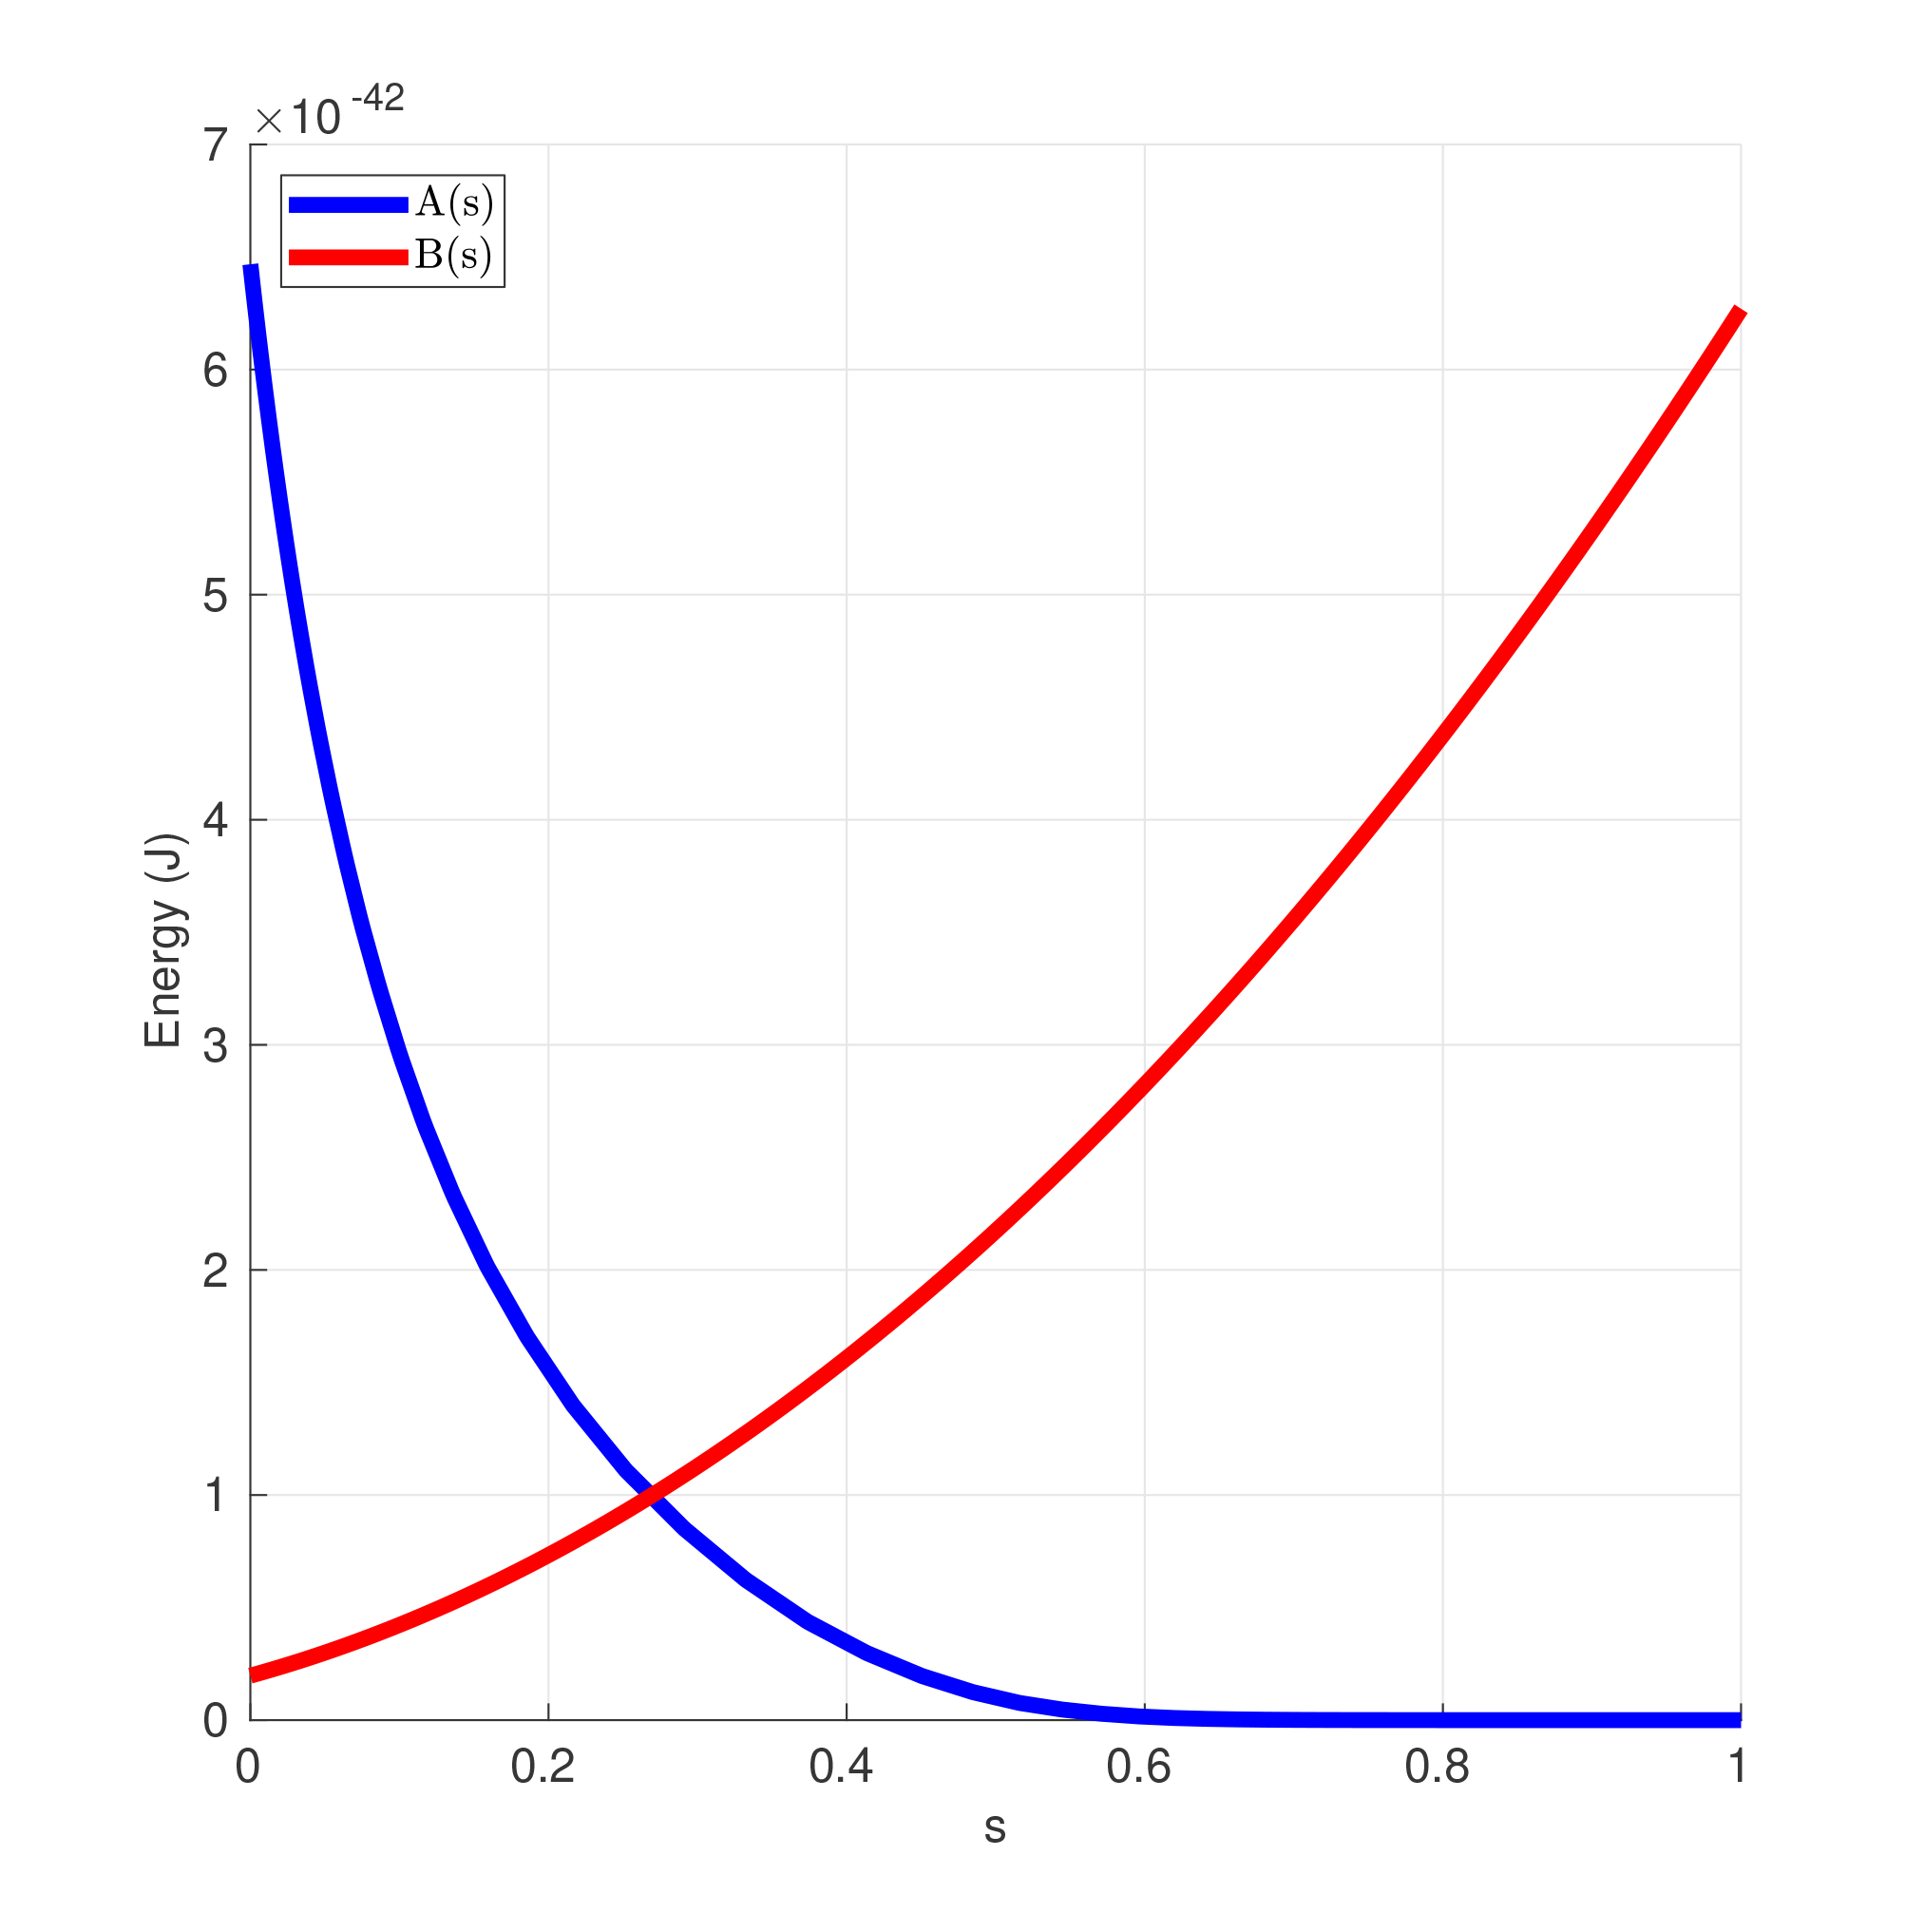
\includegraphics[scale=.14]{dwave-annealing-functions.png}
	\centering
	\caption{Annealing functions for the D-Wave 2X systems \cite{DWaveDoc-QuantumAnnealing}}
	\label{fig:dwave-annealing-functions}
\end{figure}

With these restrictions on the annealing functions, the system's Hamiltonian satisfies $H(0) = H_{initial}$ and $H(1) = H_{final}$. Therefore, the ground state at time $s=0$ matches the ground state of the initial Hamiltonian, and at time $t=1$, it matches the final Hamiltonian one. Under adiabatic evolution hypothesis, if the system starts in the initial Hamitolnian's ground state, it will end up in the final Hamiltonian one -which encodes the solution to our problem- at the end of the annealing.

The question remaining is, are the adiabatic evolution hypothesis met? We may control the time that the annealing takes by adjusting our annealing functions, a few microseconds are enough in most cases, but the exact time that would make the annealing adiabatic is never known. The additional hypothesis of the adiabatic theorem (\ref{th:adiabatic-theorem}) mentions the gap between the ground energy and the rest of eigenenergies. Let us look at a visual representation of the evolution of the eigenenergies of a given system against time in figure \ref{fig:dwave-eigenspectrum}.

\begin{figure}[h]
	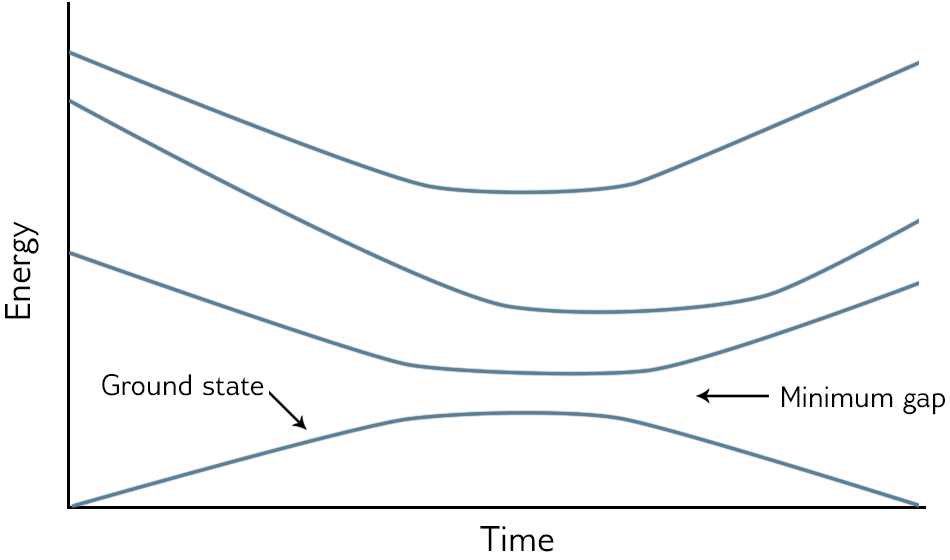
\includegraphics[scale=.3]{dwave-eigenspectrum.png}
	\centering
	\caption{Example of eigenspectrum evolution \cite{DWaveDoc-QuantumAnnealing}}
	\label{fig:dwave-eigenspectrum}
\end{figure}

The ground energy is plotted at the bottom. While the eigenenergies are far (the minimum gap holds), the probability of the system state jumping to another eigenstate is really low. When time elapses, the ground energy gets increasingly closer to the rest of the eigenenergies. The closer those energies are, the higher the probability of the system state jumping gets too. For every problem, there is a different Hamiltonian and, consequently, a different corresponding eigenspectrum. Generally, the most difficult problems for quantum annealing are those with really small minimum gaps.

In practice, these jumps may occur due to certain factors like thermal fluctuations or running the annealing process too quickly. Either way, a complete adiabatic process in the real world would mean perfect isolation, which is impossible. For some problems, the probability of staying in the ground state is really low, although low-energy states are also useful since they are associated to solutions with a low value in our cost function.


\subsection{D-Wave's QPU Topologies}
\label{sec:topologies}


In table \ref{tab:dwave-comp}, we saw the number of qubits and couplers of each one of the D-Wave QPUs. These QPUs implement a graph topology where the nodes are qubits and the couplers are the edges connecting two nodes together. However, a complete $n$-nodes graph has $n(n-1)$ nodes, and none of the D-Wave QPUs have as many couplers. For instance, the D-Wave 2000Q has $2048$ qubits and $6016$ couplers, far from the $2048 * 2047 = 4,192,256$ edges that it could have. Let us explore the graph topology underneath these systems in order to understand their problems and how to work around them.

There are two different topologies being used in the D-Wave systems. The \emph{Chimera} topology was used up until the D-Wave 2000Q system, include; while the \emph{Pegasus} topology is only in the recent Advantage system. 

In the \textbf{Chimera topology}, qubits are 'oriented' either horizontally or vertically, as seen in figure \ref{fig:chimera}.

\begin{figure}[h]
	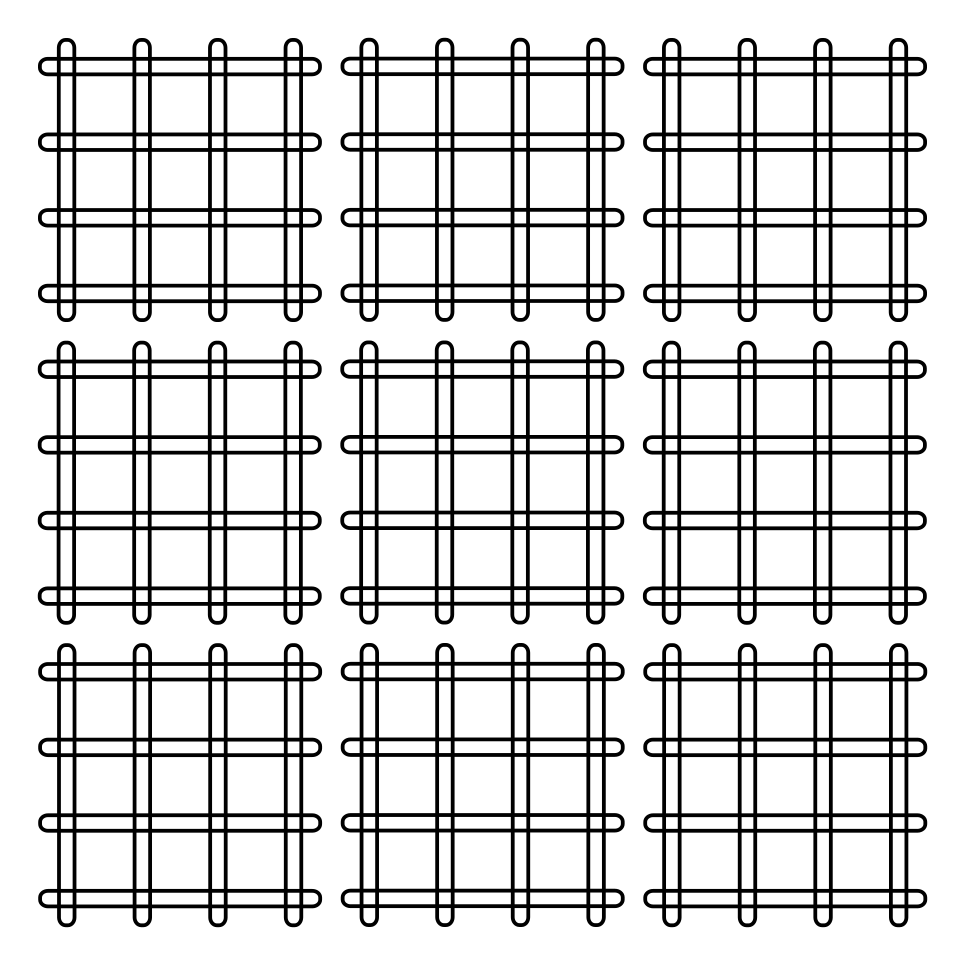
\includegraphics[scale=.3]{chimera.png}
	\centering
	\caption{Qubits represented as horizontal and vertical loops. This graphic shows three rows of 12 vertical qubits and three columns of 12 horizontal qubits for a total of 72 qubits, 36 vertical and 36 horizontal. \cite{DWaveDoc-Architecture}}
	\label{fig:chimera}
\end{figure}

For this topology it is conceptually useful to split couplers into two categories: Internal and external couplers. The \textbf{internal couplers} connect pair of orthogonal qubits. For example, in figure \ref{fig:chimera-internal-couplers} we see a green qubit connected to four black qubits through internal couplers.

\begin{figure}[H]
	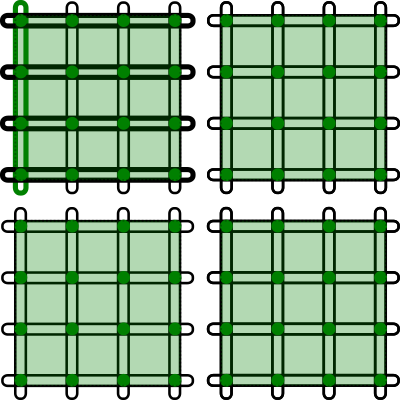
\includegraphics[scale=.5]{chimera-internal-couplers.png}
	\centering
	\caption{Internal couplers, represented as green dots at the intersections between qubits \cite{DWaveDoc-Architecture}}
	\label{fig:chimera-internal-couplers}
\end{figure}

The Chimera topology has a repetitive structure where sets of $4$ by $4$ qubits are grouped together. These are the translucent green squares in figure \ref{fig:chimera-internal-couplers} and are called \emph{unit cells}.

A unit cell can also be represented either as a cross or a column, as shown in figure \ref{fig:chimera-unit-cell}. They are $K_{4,4}$ bipartite graphs. Meaning, there are two sets of $4$ qubits, qubits on a given set are connected to every qubit in the opposite set and have no more connections. same set but are connected to every qubit of the other one. For example, the green qubit labeled as $0$ is connected to all the nodes from the opposing set: $(4,5,6,7)$.

\begin{figure}[h]
	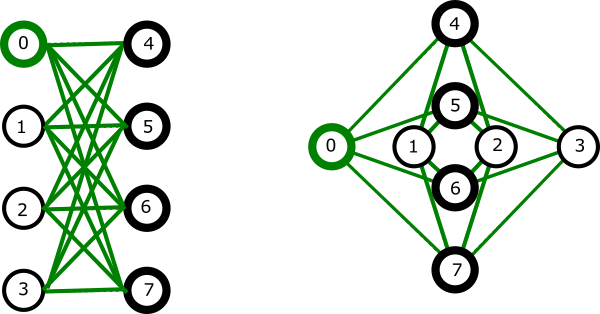
\includegraphics[scale=.7]{chimera-unit-cell.png}
	\centering
	\caption{Chimera unit cells \cite{DWaveDoc-Architecture}}
	\label{fig:chimera-unit-cell}
\end{figure}

The \textbf{external} couplers connect pairs of qubits in the same row or column, but from different unit cells. For example, in figure \ref{fig:chimera-external-couplers} the green qubit in the center unit cell is connected to the two blue qubits in other unit cells and two four black qubits in the same unit cell.

\begin{figure}[h]
	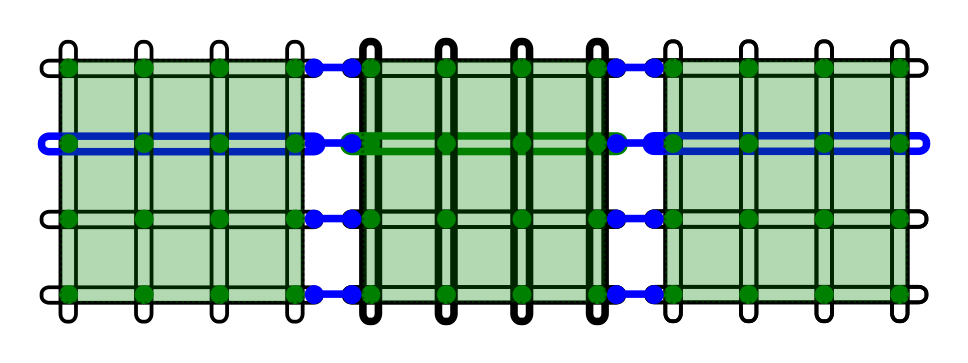
\includegraphics[scale=.5]{chimera-external-couplers.png}
	\centering
	\caption{External couplers, represented as blue connections between qubits \cite{DWaveDoc-Architecture}}
	\label{fig:chimera-external-couplers}
\end{figure}

Chimera qubits have:

\begin{itemize}
	\item A \emph{nomial length} of $4$. That is, each qubit is connected to $4$ orthogonal qubits via internal couplers.
	\item A \emph{degree} of $6$. That is, is qubit is connected to a total of $6$ other qubits.
\end{itemize}

The $K_{4,4}$ unit cells are connected by external couplers forming what is called a lattice. For instance, figure \ref{fig:chimera-extended} shows four connected unit cells that are part of a bigger topology. The notation $C_n$ refers to a chimera grid with an $N \times N$ grid of unit cells. Figure \ref{fig:chimera-internal-couplers} shows a $C_2$. The D-Wave 2000Q QPU supports a $C_16$ chimera graph.

\begin{figure}[h]
	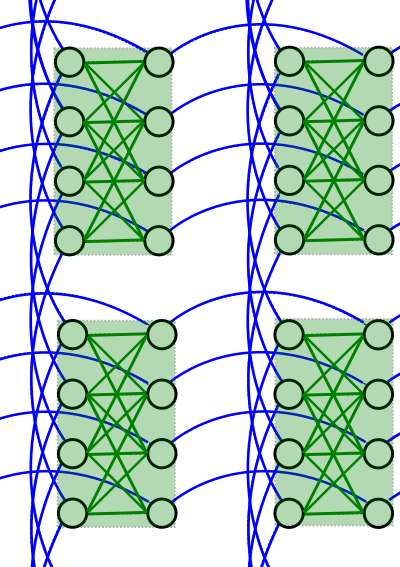
\includegraphics[scale=.4]{chimera-extended.png}
	\centering
	\caption{Cropped view of four unit cells, part of a bigger Chimera graph \cite{DWaveDoc-Architecture}}
	\label{fig:chimera-extended}
\end{figure}

The \textbf{Pegasus topology} is also organized in horizontal and vertical qubits, but they are shifted, as shown in figure \ref{fig:pegasus}. Conceptually, the chimera and the pegasus topology are not that different: the graph is divided into unit cells, connected between them using external couplers. However, a new kind of coupler is introduced in the Pegasus topology: the odd coupler.

\begin{figure}[h]
	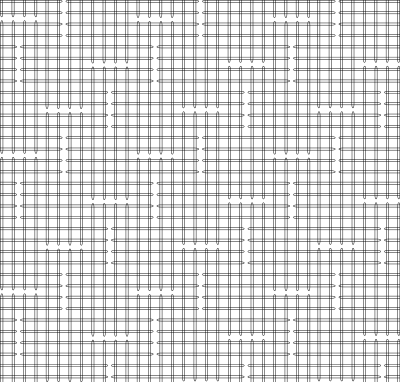
\includegraphics[scale=.08]{pegasus.png}
	\centering
	\caption{Pegasus graph \cite{DWaveDoc-Architecture}}
	\label{fig:pegasus}
\end{figure}

We will not deepen anymore into the Pegasus graph structure. It suffices to know that pegasus qubits have a nominal length of $12$ (each qubit is connected to $12$ orthonormal qubits using internal couplers) and a total degree $15$. A Pegasus cell contains $24$ qubits. Additionally, $P_n$ represents a Pegasus topology with an $N \times N$ grid of unit cells. The Advantage system supports a $P_{16}$ Pegasus graph.


\subsection{Embeddings}
\label{sec:embeddings}

Let us explore the main disadvantages of these topologiesand how to overcome them. Consider a simple example with three binary variables $(a, b, c)$: find a configuration for the variables such that $a + b + c = 1$.

This simple satisfability problem can be transform using the energy function $E(x) = (1 - a - b - c)^2$, or equivalenty $E(x) = 2ab + 2ac + 2bc - a - b - c + 1$. This matches the following QUBO model:

$$ \text{Minimize } E(x) = x^T Q x + 1$$

where

$$
Q = 
\left(
\begin{array}{ccc}
	-1 & 1 & 1  \\
	1 & -1 & 1  \\
	1 & 1 & -1
\end{array}
\right), \quad
x = 
\left(
\begin{array}{c}
a  \\
b  \\
c
\end{array}
\right)
$$

This can be seen as the graph in figure \ref{fig:example-embedding}. Suppose we want to use a Chimera topology to solve this problem. The remaining question is how to embed this graph into a chimera unit cell such as \ref{fig:chimera-unit-cell-cross}. 

\begin{figure}[H]
	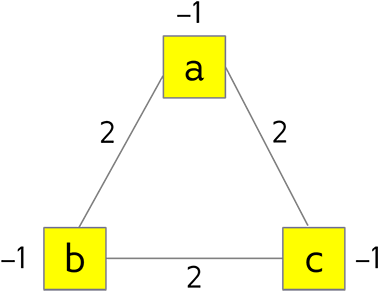
\includegraphics[scale=.3]{example-embedding.png}
	\centering
	\caption{Graph associated to QUBO model \cite{DWaveDoc-MinorEmbedding}}
	\label{fig:example-embedding}
\end{figure}

\begin{figure}[H]
	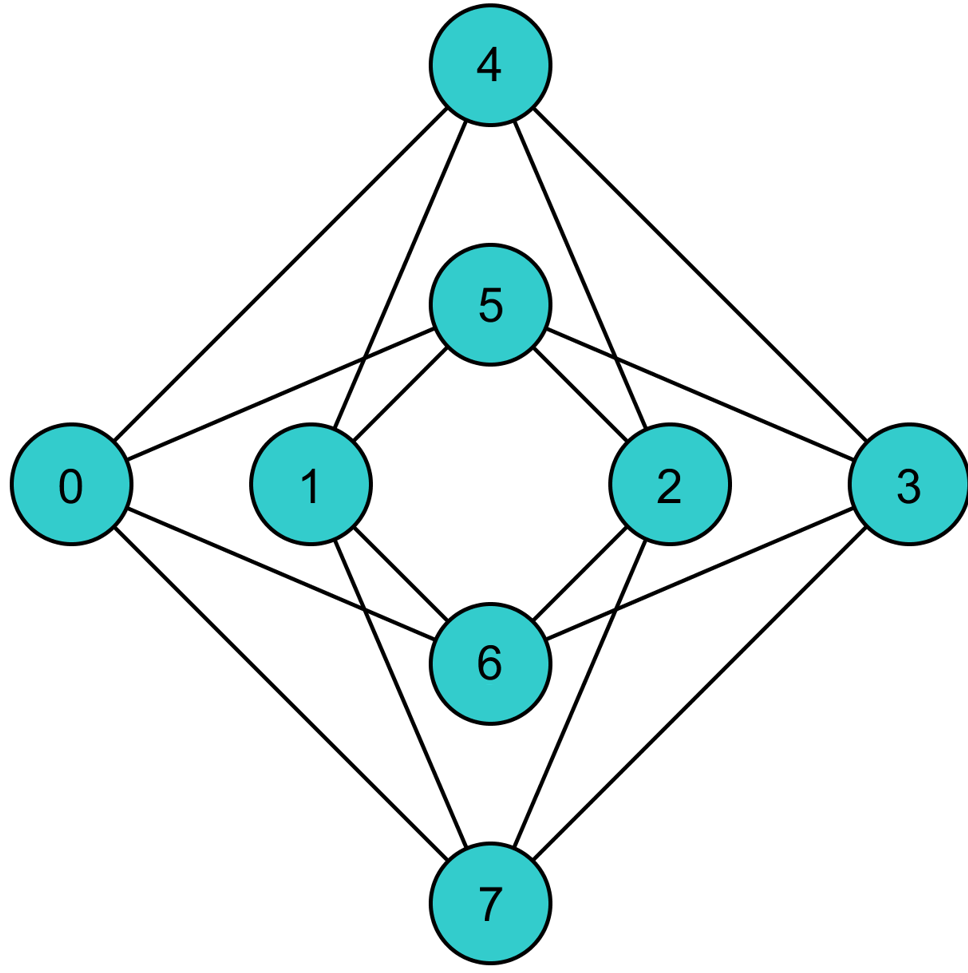
\includegraphics[scale=.2]{chimera-unit-cell-cross.png}
	\centering
	\caption{Chimera unit cell \cite{DWaveDoc-MinorEmbedding}}
	\label{fig:chimera-unit-cell-cross}
\end{figure}

However, there are no three nodes in a bipartite graph that form a triangle, so a direct embedding is not possible. Instead, a \emph{chain} is used: adjacent qubits are group together and conceptually assigned to a single node of our QUBO model graph. This process is shown in figure \ref{fig:embedding}. In practice, the coupler between qubits in a chain is set to a great negative value so the probability of both qubits ending up in the same state is really high. In most complex cases we will not manually embed a graph since D-Wave provides an automatic way of computing an (at least) suboptimal embedding.

\begin{figure}[H]
	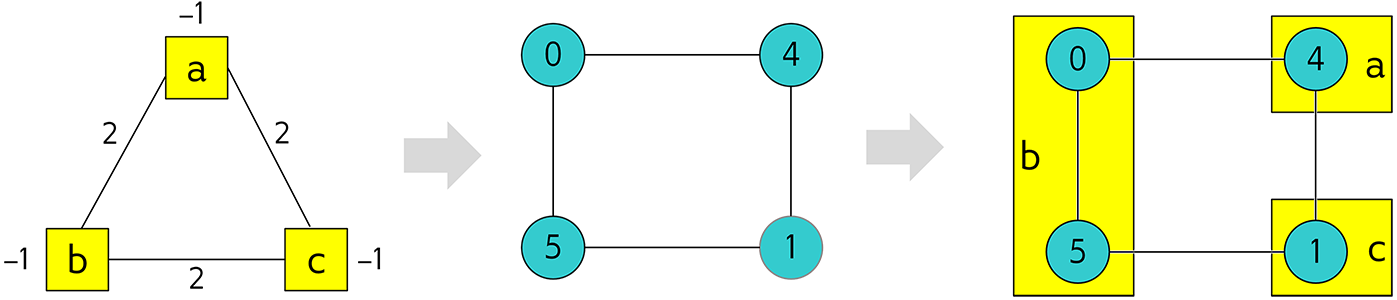
\includegraphics[scale=.3]{embedding.png}
	\centering
	\caption{Embedding process \cite{DWaveDoc-MinorEmbedding}}
	\label{fig:embedding}
\end{figure}
